\documentclass[final]{sig-alternate-05-2015}

\usepackage{url}                  % format URLs
\usepackage{listings}          % format code
\lstset{
  mathescape, 
  language={C},
  basicstyle=\small
}
\usepackage{enumitem}      % adjust spacing in enums
\usepackage[colorlinks=true,allcolors=blue,breaklinks,draft=false]{hyperref}   
\usepackage{graphicx}
\usepackage{float}
\usepackage{subcaption}
\usepackage{xspace,framed}
\usepackage{colortbl}
\usepackage{calc}
\usepackage[dvipsnames]{xcolor}
\usepackage{amssymb,amsmath,amsfonts} 
\usepackage{mathtools}
\usepackage{microtype}

\usepackage{algorithm}
\usepackage{amsfonts}
\usepackage{multicol}
\usepackage{multirow}
\usepackage{tikz}
\usetikzlibrary{positioning, automata, shapes.arrows, calc, shapes, arrows}
\usetikzlibrary{patterns}
\usepackage[justification=centering]{caption}
\usepackage{stmaryrd}
\usepackage{hhline}
\usepackage{pifont}
\usepackage{longtable}
\usepackage{afterpage}
\usepackage{wasysym}
\usepackage[scaled]{helvet}

%\usetikzlibrary{decorations}
%\usetikzlibrary{decorations.pathmorphing}

\newcommand{\aabatecmt}[1]{{\color{red}#1}}
\newcommand{\dariocmt}[1]{{\color{blue}#1}}

\newcommand{\blue}[1]{{\color{blue}#1}}
\newcommand{\red}[1]{{\color{red}#1}}
\newcommand{\green}[1]{{\color{green}#1}}
%\newcommand{\blue}[1]{}
%\newcommand{\red}[1]{}
%\newcommand{\green}[1]{}

\newtheorem{myassumption}{Assumption}
\newtheorem{mylemma}{Lemma}
\newtheorem{myprop}{Proposition}

\renewcommand{\baselinestretch}{0.99}
\allowdisplaybreaks
\newcommand{\lcsay}[1]{{\color{Magenta} LC: {#1}}} 
\newcommand{\dcsay}[1]{{\color{purple} DC: {#1}}}
\newcommand{\dksay}[1]{{\color{blue} DK: {#1}}}  
\newcommand{\aasay}[1]{{\color{red} AA: {#1}}} 
\newcommand{\cdsay}[1]{{\color{Mahogany} CD: {#1}}} 
\newcommand{\pksay}[1]{{\color{RoyalBlue} PK: {#1}}} 
\newcommand{\ibsay}[1]{{\color{Sepia} IB: {#1}}} 

\newcommand{\param}[2]{\ensuremath{\langle{#1},{#2}\rangle}\xspace}
\newcommand{\xmark}{\ding{55}}
\newcommand{\tbmark}{\hspace{-1.2em}$^*$}


\begin{document}

\CopyrightYear{2017}
\setcopyright{acmcopyright}
\conferenceinfo{HSCC '17,}{April 18--20, 2017, Pittsburgh, PA, USA.}
\isbn{978-1-4503-4590-3/17/04}\acmPrice{\$15.00.}
\doi{TBD.}

\title{
Sound and Automated Synthesis of Digital Stabilizing Controllers for Continuous
Plants%
\thanks{Supported by EPSRC grant EP/J012564/1,
ERC project 280053 (CPROVER) and the H2020 FET OPEN SC$^2$.}}

%\subtitle{[Extended Abstract]
%\titlenote{A full version of this paper is available as
%\textit{Author's Guide to Preparing ACM SIG Proceedings Using
%\LaTeX$2_\epsilon$\ and BibTeX} at
%\texttt{www.acm.org/eaddress.htm}}}
%
% You need the command \numberofauthors to handle the 'placement
% and alignment' of the authors beneath the title.
%
% For aesthetic reasons, we recommend 'three authors at a time'
% i.e. three 'name/affiliation blocks' be placed beneath the title.
%
% NOTE: You are NOT restricted in how many 'rows' of
% "name/affiliations" may appear. We just ask that you restrict
% the number of 'columns' to three.
%
% Because of the available 'opening page real-estate'
% we ask you to refrain from putting more than six authors
% (two rows with three columns) beneath the article title.
% More than six makes the first-page appear very cluttered indeed.
%
% Use the \alignauthor commands to handle the names
% and affiliations for an 'aesthetic maximum' of six authors.
% Add names, affiliations, addresses for
% the seventh etc. author(s) as the argument for the
% \additionalauthors command.
% These 'additional authors' will be output/set for you
% without further effort on your part as the last section in
% the body of your article BEFORE References or any Appendices.

%\numberofauthors{8} %  in this sample file, there are a *total*
% of EIGHT authors. SIX appear on the 'first-page' (for formatting
% reasons) and the remaining two appear in the \additionalauthors section.
%
%% \author{
%% % You can go ahead and credit any number of authors here,
%% % e.g. one 'row of three' or two rows (consisting of one row of three
%% % and a second row of one, two or three).
%% %
%% % The command \alignauthor (no curly braces needed) should
%% % precede each author name, affiliation/snail-mail address and
%% % e-mail address. Additionally, tag each line of
%% % affiliation/address with \affaddr, and tag the
%% % e-mail address with \email.
%% %
%% % 1st. author
%% \alignauthor
%% Ben Trovato\titlenote{Dr.~Trovato insisted his name be first.}\\
%%        \affaddr{Institute for Clarity in Documentation}\\
%%        \affaddr{1932 Wallamaloo Lane}\\
%%        \affaddr{Wallamaloo, New Zealand}\\
%%        \email{trovato@corporation.com}
%% % 2nd. author
%% \alignauthor
%% G.K.M. Tobin\titlenote{The secretary disavows
%% any knowledge of this author's actions.}\\
%%        \affaddr{Institute for Clarity in Documentation}\\
%%        \affaddr{P.O. Box 1212}\\
%%        \affaddr{Dublin, Ohio 43017-6221}\\
%%        \email{webmaster@marysville-ohio.com}
%% }

\author{Alessandro Abate$^{1}$, Iury Bessa$^{2}$, Dario Cattaruzza$^{1}$, Lucas Cordeiro$^{1,2}$, \\ 
Cristina David$^{1}$, Pascal Kesseli$^{1}$ and Daniel Kroening$^{1}$
\and
$^{1}$\affaddr{University of Oxford, Oxford, United Kingdom} \quad
$^{2}$\affaddr{Federal University of Amazonas, Manaus, Brazil}
}


\newcommand\tool{{\sf DSSynth}\xspace}

\maketitle

\begin{abstract}
%
Modern control is implemented with digital microcontrollers, embedded within
a dynamical plant that represents physical components.
%
We present a new algorithm based on counter\-example guided inductive
synthesis that automates the design of digital controllers that are
correct by construction.  The synthesis result is sound with respect to the
complete range of approximations, including time discretization,
quantization effects, and finite-precision arithmetic and its
rounding errors.
%
We have implemented our new algorithm in a tool called \tool, and are able
to automatically generate stable controllers for a set of intricate plant
models taken from the literature within minutes.
%
\end{abstract}

%
%  Use this command to print the description
%
\printccsdesc

% We no longer use \terms command
%\terms{Theory}

\keywords{Digital control synthesis, CEGIS, finite-word-length representation, time sampling, quantization}

%%%%%%%%%%%%%%%%%%%%%%%%%%%%%%%%%%%%%%%%%%%%%%%%%%%%%%%%%%%%%%%%%%%%%%%%%%%%%%%%%%%%%%
\section{Introduction}

Modern implementations of embedded control systems have proliferated with
the availability of low-cost devices that can perform highly non-trivial
control tasks, with significant impact in numerous application areas such as
environmental control and robotics~\cite{astrom1997computer, Franklin15}. 
Correct control is non-trivial, however.  The problem is exacerbated by
artefacts specific to digital control, such as the effects of
finite-precision arithmetic, time discretization, and quantization noise
introduced by A/D and D/A conversion.  Thus, programming expertise is a key
barrier to broad adoption of correct digital controllers, and requires
considerable knowledge outside of the expertise of many control engineers.

Beyond classical a-posteriori validation in digital control, there has been
plenty of previous work aiming at \emph{verifying} a given designed
controller, which however broadly lack automation.  Recent work has studied
the stability of digital controllers considering implementation aspects,
i.e., fixed-point arithmetic and the word length~\cite{Bessa16}.  They
exploit advances in bit-accurate verification of C programs to obtain a
verifier for software-implemented digital control.

By contrast, we leverage a very recent step-change in the automation and
scalability of \emph{program synthesis}.  Program synthesis engines use a
specification as the starting point, and subsequently generate a sequence of
candidate programs from a given template.  The candidate programs are
iteratively refined to eventually satisfy the specification.  Program
synthesizers implementing Counter-Example Guided Inductive Synthesis
(CEGIS)~\cite{sketch} are now able to generate programs for highly
non-trivial specifications with a very high degree of automation.  Modern
synthesis engines combine automated testing, genetic algorithms, and
SMT-based automated reasoning~\cite{DBLP:journals/corr/AlurFSS16a,
DBLP:conf/lpar/DavidKL15}.

By combining and applying state-of-the-art synthesis engines we present a
tool that automatically generates digital controllers for a given continuous
plant model that are correct by construction.  This approach delivers a high
degree of automation, promises to reduce the cost and time of development of
digital control dramatically, and requires considerably less expertise than
a-posteriori verification.  Specifically, we synthesize stable,
software-implemented embedded controllers along with a model of a physical
plant.  Due to the complexity of such closed-loop systems, in this work we
focus on linear models with known configurations, and perform parametric
synthesis of stabilizing digital controllers (further closed-loop
requirements are left to future work).

Our work addresses challenging aspects of the control synthesis problem.  We
perform digital control synthesis over a hybrid model, where the plant
exhibits continuous behavior whereas the controller operates in discrete
time and over a quantized domain.  Inspired by a classical
approach~\cite{astrom1997computer}, we translate the problem into a single
digital domain, i.e., we model a digital equivalent of the continuous plant
by evaluating the effects of the quantizers (A/D and D/A converters) and of
time discretization.  We further account for uncertainties in the plant
model.  The resulting closed-loop system is a program with a loop that
operates on bit-vectors encoded using fixed-point arithmetic with finite
word length (FWL).  The three effects of 1.~uncertaities, 2.~FWL
representation and 3.~quantization errors are incorporated into the model,
and are taken into account during the CEGIS-based synthesis of the control
software for the plant.

In summary, this paper makes the following original contributions.
%
\begin{itemize}

\item We automatically generate {\em correct-by-construction} digital
  controllers using an inductive synthesis approach.  Our application of program
  synthesis is non-trivial and addresses challenges specific to control
  systems, such as the effects of quantizers and FWL.  In particular, we
  have found that a two-stage verification engine that continuously refines
  the precision of the fixed-point representation of the plant yields a
  speed-up of two orders of magnitude over a conventional one-stage
  verification engine.

\item Experimental results show that \tool is able to efficiently synthesize
  stable controllers for a set of intricate benchmarks taken from the
  literature: the median runtime for our benchmark set considering the
  faster engine is $48$\,s, i.e., half of the controllers can be synthesized
  in less than one minute.

%% \item We exploit a CEGIS-based approach that uses inductive synthesis
%% together with a bit-precise formal verification algorithm for synthesizing
%% correct-by-design robust digital controllers for non-fragile closed-loop
%% stability.

%% \item Experimental results with our synthesizer show that the
%% combination of interval arithmetic to represent the controller coefficients
%% and a two-stage verification approach to continuously refine precision
%% enables us to compute a parametric, sound solution for $14$ out of $15$
%% digital stabilizing controllers for a set of continuous and discrete plants
%% with parametric uncertainties.

\end{itemize}

%\begin{figure}
%\centering
%\resizebox{.35\textwidth}{!}{
% \begin{tikzpicture}[scale=0.3,-,>=stealth',shorten >=.2pt,auto,
%     semithick, initial text=, ampersand replacement=\&,]

%  \matrix[nodes={draw, fill=none, shape=rectangle, minimum height=.2cm, minimum width=.2cm, align=center}, row sep=.5cm, column sep=.5cm] {
%   \coordinate (aux0);
%   \& \node[circle] (circle) {}; 
%   \& \node[fill=yellow!20] (da) {{\sc D/A}}; 
%   \& \node[fill=yellow!20] (p) {{\sc P}};
%   \& \node[fill=yellow!20] (ad) {{\sc A/D}}; 
%   \& \coordinate (aux1);\\
%   \& \coordinate (aux3); 
%   \&
%   \&
%   \node[fill=yellow!20] (c) {C};
%   \& 
%   \& \coordinate (aux2);\\
%  };


%  \path[->] (aux0) edge (circle.west);
%  \path  
%   (circle.east) edge (da.west)
%   (da.east) edge (p.west)
%   (p.east) edge (ad.west)
%   (ad.east) edge (aux1.west)
%   (aux1.south) edge (aux2.north)
%   (aux2.west) edge (c.east)
%   (c.west) edge (aux3.east); 
%  \path[->]  (aux3.north) edge (circle.south);
% \end{tikzpicture}
%}
% \caption{Closed-Loop System. \label{fig:closed-system}}
%\end{figure}

%\textcolor{cyan}{[if space is needed, the next paragraph can be cut. ]}
%We cover preliminaries on plant discretization, the verification of
%closed-loop control systems, and stability in
%Section~\ref{sec:preliminaries}.  Our core contribution is in
%Section~\ref{sec:synthesis}: we present our CEGIS-based algorithm for
%generating stable controllers for a given plant model.  Our experimental
%setup and experimental results are given in Section~\ref{sec:experiments},
%and we discuss how we extend the state-of-the-art beyond the existing
%literature in Section~\ref{sec:related}.

%%%%%%%%%%%%%%%%%%%%%%%%%%%%%%%%%%%%%%%%%%%%%%%%%%%%%%%%%%%%%%%%%%%%%%%%%%%%%%%%%%%%%%
\section{Preliminaries}\label{sec:preliminaries}

%------------------------------------
\subsection{Discretization of the Plant}
\label{ssec:SandH}
%------------------------------------

The digital controllers synthesized using the algorithm we present in this
paper are typically used in closed loops with continuous (physical) plants. 
Thus, we consider continuous dynamics (the plant) and discrete parts (the
digital controller). In order to obtain an overall model, we discretize the
continuous plant and look at the plant dynamics from the perspective of the digital controller. 

As we only consider transfer function models, and require a $z$-domain transfer
function $G(z)$ that captures all aspects of the continuous plant, 
which is naturally described via a Laplace-domain transfer function $G(s)$. 
The continuous model of the plant must be discretized to obtain the
corresponding coefficients of $G(z)$.

Among the discretization methods in the literature~\cite{Franklin15}, 
we consider the sample-and-hold processes in complex systems~\cite{istepanian2012digital}.  
On the other hand, 
the ZOH discretization models the exact effect of sampling and DAC interpolation over the plant.

\begin{myassumption}
%
The sample-and-hold effects of the ADC and the presence of the ZOH of the DAC are synchronized,
namely there is no delay between sampling the plant output at the ADC and
updating the DAC accordingly.  The DAC interpolator is an ideal ZOH. 
%
\end{myassumption}

\begin{mylemma}\cite{astrom1997computer}
%
Given a synchronized ZOH input and sample-and-hold output on the plant, 
with a sample time $T$ satisfying the Nyquist criterion, the discrete pulse
transfer function $G(z,T)$ is an exact z-domain representation of $G(s)$, 
and can be computed using the following formula:
%
\begin{equation}
\label{eq:pulsetf}
G(z,T) = %\mathcal{ZOH}\left\lbrace{G(s)}\right\rbrace =
(1-z^{-1})\mathcal{Z}\left\lbrace{\mathcal{L}^{-1}\left\lbrace{\frac{G(s)}{s}}\right\rbrace_{t=kT}}\right\rbrace.
\end{equation}
%
\end{mylemma}
%
For the sake of brevity, we will use the notation $G(z)$ to represent the
pulse transfer function $G(z,T)$.
% 
Lemma~\ref{eq:pulsetf} ensures that the poles and zeros match under the
$\mathcal{Z}\left\lbrace{\mathcal{L}^{-1}\left\lbrace{\cdot}\right\rbrace_{t=kT}}\right\rbrace$
operations, and it includes the ZOH dynamics in the $(1-z^{-1})$ term.  This
is sufficient for stability studies over $G(s)$~\cite{fadali}, i.e., if
there is any unstable pole (in the complex domain $\Re\{s\} > 0$), the pulse
transfer function in~\eqref{eq:pulsetf} will also present the same number of
unstable poles ($|z| > 1$)~\cite{Franklin15}.

%------------------------------------
\subsection{Model Imprecision, Finite Word Length Representation and Quantization Effects}
\label{verifying-closed-loop-control-systems}
%------------------------------------

Let $C(z)$ be a digital controller and $G(z)$ be a discrete-time representation of the plant, 
given as
%
\begin{align}
\small
\label{controller_plant_tf}
C(z)&=\frac{C_n(z)}{C_d(z)}=\frac{\beta_{0}+\beta_{1}z^{-1}+...+\beta_{M_C}z^{-M_C}}{\alpha_{0}+\alpha_{1}z^{-1}+...+\alpha_{N_C}z^{-N_C}}, \\
%\label{plant_tf}
G(z)&=\frac{G_n(z)}{G_d(z)}=\frac{b_{0}+b_{1}z^{-1}+...+b_{M_G}z^{-M_G}}{a_{0}+a_{1}z^{-1}+...+a_{N_G}z^{-N_G}}.
\end{align}
%
where $\vec{\beta}$ and $\vec{\alpha}$ are vectors containing the
controller's coefficients; similarly, $\vec{b}$ and $\vec{a}$ denote the
plant's coefficients; 
and finally $N_{(\cdot)}$ and $M_{(\cdot)}$ indicate the order of the polynomials,  
and we require in particular that $N_G \geq M_G$. 

Uncertainties in $G(z)$ may appear owing to: 1.~uncertainties in $G(s)$ (we
denote the uncertain continuous plant by
$\hat{G}(s)=\frac{G_n(s)+\Delta_p{G}_n(s)}{G_d(s)+\Delta_p{G}_d(s)}$ to
explicitly encompass the effects of the uncertainty terms
$\Delta_p{G}_{(\cdot)}(s)$) arising from tolerances/imprecision in the
original model; 2.~errors in the numerical calculations due to FWL effects
(e.g., coefficient truncation and round-off, which will be denoted as
$\Delta_b{G}_n(s),\Delta_b{G}_d(s)$); and 3.~errors caused by quantization
(which we model later as as external disturbances $\nu_1$ and $\nu_2$). 
These uncertainties are parametrically expressed by additive terms,
eventually resulting in an uncertain model $\hat{G}(z)$, such that:
%
\begin{equation}
\hat{G}(z)=\frac{G_n(z)+\Delta G_n(z)}{G_d(z)+\Delta G_d(z)},
\end{equation}
%
%\red{[what is the relationship between the deltas in this formula, and those in the previous paragraph? please clarify and hopefully simplify formulae. ]}
which will be represented by the following transfer function:
%
\begin{equation}
\hat{G}(z)=\frac{\hat{b}_{0}+\hat{b}_{1}z^{-1}+...+\hat{b}_{M_G}z^{-M_G}}{\hat{a}_{0}+\hat{a}_{1}z^{-1}+...+\hat{a}_{N_G}z^{-N_G}}. 
\end{equation}
%
Notice that, due to the nature of the methods we use for the stability
check, we require that the parametric errors in the plant have the same
polynomial order as the plant itself (indeed, all other errors described in
this paper fulfil this property).  We~also remark that, due to its native
digital implementation, there are no parametric errors ($\Delta_pC_n(z),
\Delta_pC_d(z)$) in the controller.  Thus $\hat{C}(z) \equiv C(z)$.

We introduce next a notation based on the polynomials coefficients to simplify 
the presentation.  Let $\mathcal{P}^{N}$ be the space of polynomials of order $N$. 
Let $P \in \mathcal{P}^{M,N}$ be a rational polynomial 
$\frac{P_n}{P_d}$, where $P_n \in \mathcal{P}^{M}$ and $P_d \in \mathcal{P}^{N}$.  
For a vector of coefficients
%
\begin{equation}
\vec{P} \in \mathbb{R}^{N+M+2}=[n_{0}\ n_{1}\ \hdots \ n_{M}\ d_{0}\ d_{1}\ \hdots\ d_{N}\ ]^T
\label{eq:coefficients}
\end{equation}
%
and an uncertainty vector 
%
\begin{equation}
\Delta{\vec{P}}\in \mathbb{R}^{N+M+2}=[\Delta{n}_{0}\ \hdots \ \Delta{n}_{M}\ \Delta{d}_{0}\ \hdots\ \Delta{d}_{N}\ ]^T \; 
\label{eq:delta_coefficients}
\end{equation}
%
we write
\begin{align}
\label{eq:hatgvector}
\vec{\hat{G}}&=\vec{G}+\Delta{\vec{G}}, \text{ where} \\
\vec{G} \in \mathbb{R}^{N_G+M_G+2}&=[b_{0}\ \hdots \ b_{M_G}\ a_{0}\ \hdots\ a_{N_G}\ ]^T, \nonumber \\
\Delta{\vec{G}}\in \mathbb{R}^{N_G+M_G+2}&=[\Delta{b}_{0}\ \hdots \ \Delta{b}_{M_G}\ \Delta{a}_{0}\ \hdots\ \Delta{a}_{N_G}\ ]^T. \nonumber
\end{align}
In the following we will either manipulate the transfer functions $G(z)$, $C(z)$ directly, 
or work over their respective coefficients $\vec{G}$, $\vec{C}$ in vector form.

\medskip

\begin{figure*}[htb]
\centering

\tikzset{add/.style n args={4}{
    minimum width=6mm,
    path picture={
        \draw[circle] 
            (path picture bounding box.south east) -- (path picture bounding box.north west)
            (path picture bounding box.south west) -- (path picture bounding box.north east);
        \node[draw=none] at ($(path picture bounding box.south)+(0,0.13)$)     {\small #1};
        \node[draw=none] at ($(path picture bounding box.west)+(0.13,0)$)      {\small #2};
        \node[draw=none] at ($(path picture bounding box.north)+(0,-0.13)$)    {\small #3};
        \node[draw=none] at ($(path picture bounding box.east)+(-0.13,0)$)     {\small #4};
        }
    }
 }

\resizebox{1.0\textwidth}{!}{
 \begin{tikzpicture}[scale=0.6,-,>=stealth',shorten >=.2pt,auto,
     semithick, initial text=, ampersand replacement=\&,]

  \matrix[nodes={draw, fill=none, shape=rectangle, minimum height=.2cm, minimum width=.2cm, align=center}, row sep=.6cm, column sep=.6cm] {
    \node[draw=none] (r) {$R(z)$};
%   \& \coordinate (aux0);
   \& \node[circle,add={-}{+}{}{}] (circle) {};
   \node[draw=none] (ez) at ([xshift=1cm,yshift=.15cm]circle)  {$e(z)$};
   \& \node[rectangle,draw,
	minimum width=1cm,
	minimum height=1cm,
        label=\textbf{Controller}] (cz) {\sc $\hat{C}(z)$};
   \node[draw=none] (ud) at ([xshift=1cm,yshift=.15cm]cz)  {$U(z)$};
     
   \& complexnode/.pic={ 
      \node[rectangle,draw,
	minimum width=3cm,
	minimum height=1.6cm,
	label=\textbf{DAC},] (dac) {};
     \node[circle,add={}{+}{+}{},fill=gray!20] (q2) at ([xshift=-.65cm]dac.center) {};
     \node[draw=none] (q2t)  at ([xshift=-.65cm,yshift=-.65cm]dac.center) {{\sc Q2}};
     \node[draw=none] (v2)  at ([xshift=-.65cm,yshift=1.5cm]dac.center) {$\nu_2(z)$};
     \node[fill=gray!20] (zoh) at ([xshift=.65cm]dac.center) {{\sc ZOH}};}   
   \& \node[rectangle,draw,
	minimum width=1cm,
	minimum height=1cm,
        label=\textbf{Plant}] (gs) {{\sc $\hat{G}(s)$}};
   \node[draw=none] (ud) at ([xshift=-2cm,yshift=.15cm]gs)  {$U(s)$};
   \node[draw=none] (y) at ([xshift=2cm,yshift=.15cm]gs)  {$\hat{Y}(s)$};
   \& complexnode/.pic={ 
     \node[rectangle,draw,
	minimum width=4cm,
	minimum height=1.6cm,
	label=\textbf{ADC},] (adc) {};
   \draw[] ([xshift=-1cm]adc.center) -- ++(0.5,0.2cm);
   \coordinate (switch1) at ([xshift=-1cm]adc.center);
   \coordinate (switch2) at ([xshift=-0.4cm]adc.center);
   \node[circle,add={}{+}{+}{},fill=gray!20] (q1) at ([xshift=1cm]adc.center) {};} 
     \node[draw=none] (q2t)  at ([xshift=1cm,yshift=-.65cm]adc.center) {{\sc Q1}};
   \node[draw=none] (v1)  at ([xshift=1cm,yshift=1.5cm]adc.center) {$\nu_1(z)$};
   \& \coordinate (aux1);
   \& \node[draw=none] (yz) {$\hat {Y}(z)$};\\
   \& \coordinate (aux3); 
   \&
   \&
   \& 
   \& 
   \& \coordinate (aux2);\\
  };


  \path[->] (v1) edge (q1.north);
  \path[->] (v2) edge (q2.north);
  \path[->] (r) edge (circle.west);
  \path[->] (aux1) edge (yz);
  \path  
   (circle.east) edge (cz)
   (cz.east) edge (q2.west)
   (q2.east) edge (zoh.west)
   (zoh.east) edge (gs.west)
   (switch2) edge (q1.west)
   (q1.east) edge (aux1.west)
   (gs.east) edge (switch1.west)
   (aux1.south) edge (aux2.north)
   (aux2.west) edge (aux3.east); 
  \path[->]  (aux3.north) edge (circle.south);
 \end{tikzpicture}
}
 \caption{Closed-loop digital control system (cf.~Section \ref{verifying-closed-loop-control-systems} for notation) \label{fig:sampledsystem}}
\end{figure*}

A typical digital control system with a continuous plant and a discrete
controller is illustrated in Figure~\ref{fig:sampledsystem}.  The DAC and
ADC converters introduce quantization errors (notice that each of them
may have a different FWL representation than the controller),
which are modeled as disturbances 
$\nu_{1}(z)$ and $\nu_{2}(z)$;  
$G(s)$ is the continuous-time plant model
with parametric additive uncertainty $\Delta_p{G}_n(s)$ and $\Delta_p{G}_d(s)$ (as mentioned above);  
$R(z)$ is a given reference signal; 
$U(z)$ is the control signal; 
and $\hat{Y}(z)$ is the output signal affected by the disturbances and uncertainties in the closed-loop system 
%
%
%
The ADC and DAC may be abstracted by transforming the closed-loop system in
Figure~\ref{fig:sampledsystem} into the digital system in 
Figure~\ref{fig:digsystem1}, 
where 
% the parametric uncertainties are represented by~$\Delta_p \vec{G}$ and 
the effect of $\nu_{1}$ and $\nu_{2}$ in the output $Y(z)$ is
seen as additive noise.  

\begin{figure}[ht]
\centering
\tikzset{add/.style n args={4}{
    minimum width=6mm,
    path picture={
        \draw[circle] 
            (path picture bounding box.south east) -- (path picture bounding box.north west)
            (path picture bounding box.south west) -- (path picture bounding box.north east);
        \node[draw=none] at ($(path picture bounding box.south)+(0,0.13)$)     {\small #1};
        \node[draw=none] at ($(path picture bounding box.west)+(0.13,0)$)      {\small #2};
        \node[draw=none] at ($(path picture bounding box.north)+(0,-0.13)$)    {\small #3};
        \node[draw=none] at ($(path picture bounding box.east)+(-0.13,0)$)     {\small #4};
        }
    }
 }

\resizebox{.48\textwidth}{!}{
 \begin{tikzpicture}[scale=0.3,-,>=stealth',shorten >=.2pt,auto,
     semithick, initial text=, ampersand replacement=\&,]

  \matrix[nodes={draw, fill=none, shape=rectangle, minimum height=.2cm, minimum width=.2cm, align=center}, row sep=.6cm, column sep=.3cm] {
    \node[draw=none] (r) {$R(z)$};
%   \& \coordinate (aux0);
   \& \node[circle,add={-}{+}{}{}] (circle) {};
   \node[draw=none] (ez) at ([xshift=1cm,yshift=.15cm]circle)  {$e(z)$};
   \& \node[rectangle,draw,
	minimum width=1cm,
	minimum height=1cm,
        label=\textbf{Controller}] (cz) {\sc $\hat{C}(z)$};
   \node[draw=none] (ud) at ([xshift=1cm,yshift=.15cm]cz)  {$U(z)$};
   \& \node[circle,add={}{+}{+}{}] (circle2) {};
   \node[draw=none] (nu2) at ([yshift=1cm]circle2)  {$\nu_2(z)$};
   \& \node[rectangle,draw,
	minimum width=1cm,
	minimum height=1cm,
        label=\textbf{Plant}] (gs) {{\sc $\hat{G}(z)$}};
%   \node[draw=none] (y) at ([xshift=2cm,yshift=.15cm]gs)  {$Y(z)$};

   \& \node[circle,add={}{+}{+}{}] (circle3) {};
   \node[draw=none] (nu1) at ([yshift=1cm]circle3)  {$\nu_1(z)$};
   \& \coordinate (aux1);
   \& \node[draw=none] (yz) {$\hat Y(z)$};\\
   \& \coordinate (aux3); 
   \&
   \& 
   \& 
   \&
   \& \coordinate (aux2);\\
  };


%  \path[->] (v1) edge (q1.north);
%  \path[->] (v2) edge (q2.north);
  \path[->] (r) edge (circle.west);
  \path[->] (nu2) edge (circle2.north);
  \path[->] (nu1) edge (circle3.north);
  \path[->] (aux1) edge (yz);
  \path  
   (circle.east) edge (cz)
   (cz.east) edge (circle2.west)
   (circle2.east) edge (gs.west)
   (gs.east) edge (circle3.west)
   (circle3.east) edge (aux1.west)
   (aux1.south) edge (aux2.north)
   (aux2.west) edge (aux3.east); 
  \path[->]  (aux3.north) edge (circle.south);
 \end{tikzpicture}
}
\caption{Fully digital equivalent to system in Figure~\ref{fig:sampledsystem} 
\label{fig:digsystem1}}
\end{figure}

In Figure~\ref{fig:digsystem1}, two sources of uncertainty are illustrated:
parametric uncertainties related to modeling errors  
(which are represented by~$\Delta_p \vec{G}$),  
and uncertainties introduced by quantizations in the ADC and
DAC conversions ($\nu_1$ and $\nu_2$) which are assumed to be non-deterministic. 
Recall that we discussed how the quantization noise is encompassed as an additive term, 
which means it does not enter parametrically in the transfer function. 
Instead, we later show that the system is stable given these non-deterministic disturbance inputs. 

The uncertain model may be rewritten as a vector of coefficients in the 
z-domain using equation \eqref{eq:hatgvector} as  
$\vec{\hat{G}}=\vec{G}+\Delta_p \vec{G}$.
The parametric uncertainties in the plant are assumed to have the same
order as the plant model, since 
errors of higher order can move the closed-loop poles by large amounts, 
thus preventing any given controller from stabilizing such a setup. 
This is a reasonable assumption since most tolerances do not change the 
architecture of the plant. 



\smallskip

\paragraph{Direct use of controllers in fixed-point representation}

Since the controller is implemented using finite representation, $C(z)$ also suffers
disturbances from the FWL effects, with roundoffs in coefficients that may
change closed-loop poles and zeros position, and consequently affect its
stability, as argued in~\cite{Bessa16}.

Let $\hat{C}(z)$ be the digital controller transfer function represented
using this FWL with integer size $I$ and fractional size~$F$. 
The term $I$ affects the range of the representation and is set to avoid overflows, 
while $F$ affects the precision and the truncation after arithmetic operations. 
We shall denote the FWL domain of the coefficients by $\mathbb{R}\langle I,F
\rangle$ and define a function
\begin{align}
\small
%\label{FWL_tf}
\mathcal{F}_n&\param{I}{F}(P \in \mathcal{P}):\mathcal{P}^{n}\rightarrow \mathcal{P}^{n}\param{I}{F} \\
&\triangleq \tilde P \in \mathcal{P}^{n}\param{I}{F} : c_i \in \vec{P} \wedge \tilde c_i \in \vec{\tilde{P}}=\mathcal{F}_0\param{I}{F}(c_i),  \nonumber
\end{align}
where $\mathcal{P}^{n}$ is the space of polynomials of $n$-th order,
$\mathcal{P}^{n}\param{I}{F}$ is the space of polynomials with coefficients in $\mathbb{R}\param{I}{F}$, 
and (as a special case) $\mathcal{F}_0\param{I}{F}(x)$ returns the element $\tilde{x} \in \mathbb{R}\param{I}{F}$ that is closest to the real parameter $x$. 

Similarly, $\mathcal{F}_{n,m}\langle I,F \rangle(\cdot):\mathcal{P}^{n,m}\rightarrow \mathcal{P}^{n,m}\langle I,F \rangle$ applies the same effect to a ratio of polynomials, where $\mathcal{P}^{n,m}$,  $\mathcal{P}^{n,m}\langle I,F
\rangle$ are rational polynomial domains.

Thus, the perturbed controller model $\tilde{C}(z)$ may be obtained from the
original model $\hat{C}(z) = C(z) = \frac{C_{n}(z)}{C_{d}(z)}$ as follows:
%
\begin{equation}
\tilde{C}(z)=\mathcal{F}_{M_C,N_C}\param{I}{F}(C(z))=\frac{\mathcal{F}_{M_C}\param{I}{F} (\hat{C}_n(z))}{\mathcal{F}_{N_C}\param{I}{F}(\hat{C}_d(z))}.
\end{equation}
%
In the case of a digitally synthesized controller (as it is the case in this work), 
because the synthesis is performed directly using FWL representation, 
$\tilde{C}(z) \equiv \hat{C}(z) \equiv C(z)$ 
(in other words, 
we synthesise a controller that is already in the domain $\mathbb{R} \param{I}{F}$ and has therefore no uncertainties entering because of FWL representations, 
that is $\Delta_bC_n(z)=\Delta_bC_d(z)=0$).


\paragraph{Fixed-point computation in program synthesis}

The program synthesis engine uses fixed-point arithmetic.  Specifically, we
use the domain $\mathbb{R}\param{I}{F}$ for the controller's coefficients
and the domain $\mathbb{R}\param{I_p}{F_p}$ for the plant's coefficients,
where $I$ and $F$, as well as $I_p$ and $F_p$, denote the number of bits for
the integer and fractional parts, respectively, and where it is practically motivated to consider $\mathbb{R}\param{
I_p}{F_p} \supseteq \mathbb{R}\param{I}{F}$.


Given the use of fixed-point arithmetic, we examine the discretization effect 
during these operations. Let $\tilde C(z)$ and $\tilde G(z)$ be 
transfer functions represented using fixed-point bit-vectors.
%
\begin{align}
\small
\label{digital_controller_plant_tf}
\tilde C(z)&=\frac{\tilde \beta_{0}+\tilde \beta_{1}z^{-1}+...+\tilde \beta_{M_C}z^{-M_C}}{\tilde \alpha_{0}+\tilde \alpha_{1}z^{-1}+...+\tilde \alpha_{N_C}z^{-N_C}}, \\
%\label{plant_tf}
\tilde G(z)&=\frac{\tilde b_{0}+\tilde b_{1}z^{-1}+...+\tilde b_{M_G}z^{-M_G}}{\tilde a_{0}+\tilde a_{1}z^{-1}+...+\tilde a_{N_G}z^{-N_G}}.
\end{align}

Recall that since the controller is synthesized in the $\mathbb{R}\param {I}{F}$
domain, $\tilde{C}(z) \equiv \hat{C}(z) \equiv C(z)$. 
However, given a real plant $\hat{G}(z)$, 
we need to introduce $\tilde G(z)=\mathcal{F}_{M_G,N_G}\param {I_p}{F_p}(\hat{G}(z))$, where 
%
\begin{align}
\label{digital_plant_tf}
\tilde G(z)&=\frac{(\hat{b}_{0}+\Delta_b \hat{b}_{0}) +...+(\hat{b}_{M_G}+\Delta_b \hat{b}_{M_G})z^{-M_G}}{(\hat{a}_{0}+\Delta_b \hat{a}_{0})+...+(\hat{a}_{N_G}+\Delta_b \hat{a}_{N_G})z^{-N_G}} \nonumber \\
\vec{\tilde G} &=\vec{\hat{G}}+\Delta_b{\vec{G}}=\vec{G}+\Delta_p{\vec{G}}+\Delta_b{\vec{G}}, 
\end{align}
%
where $\Delta_bc_i=\tilde{c}_i-\hat{c}_i$, 
and $\Delta_b{G}$ represents the plant uncertainty caused by
the rounding off effect.  We encompass the global uncertainty as
$\Delta{\vec{G}}=\Delta_p{\vec{G}}+\Delta_b{\vec{G}}$. 

%------------------------------------
\subsection{Closed-Loop Stability Verification under Parametric Uncertainties FWL Representation, and Quantisation Noise}
\label{sec:stability}
%------------------------------------

\aabatecmt{[Dario: please go through this section again, and clarify what sources of imprecision we consider where, distinguishing between plant and controller. also comment on why we operate on hat G rather than on tilde G - as we discussed yesterday. ]}
\dariocmt{I added a paragraph at the end of the section that should clarify.}
Sound synthesis of the digital controller requires the consideration of the effect of FWL on the controller, 
and of quantization disturbances in the closed-loop system.  
Let the quantizer $Q1$ (ADC) be the source of a white noise $\nu_{1}$, 
and $Q2$ (DAC) be the source of a white noise $\nu_{2}$.  The following equation
models the system in Figure~\ref{fig:sampledsystem}, encompassing the
parametric uncertainties $\Delta \vec{G}$ and the FWL effects on
the controller $\tilde{C}(z)$:
%
\begin{equation}
\hat{Y}(z)=\nu_{1}(z)+\hat{G}(z)\tilde{C}(z)R(z)+\hat{G}(z)\nu_{2}(z)-\hat{G}(z)\tilde{C}(z)\hat{Y}(z). 
\end{equation}
%
The above can be rewritten as follows:
%
\begin{equation}
\label{eq:outputfunctions}
\hat{Y}(z)=H_{1}(z)\nu_{1}(z)+H_{2}(z)\nu_{2}(z)+H_{3}(z) R(z),
\end{equation}
%
where
%
\begin{equation*}
H_{1}(z)=\frac{1}{1+\hat{G}(z) \tilde{C}(z)}, 
\end{equation*}
%
\begin{equation*}
H_{2}(z)=\frac{\hat{G}(z)}{1+\hat{G}(z) \tilde{C}(z)}, 
\end{equation*}
%
\begin{equation*}
H_{3}(z)=\frac{\hat{G}(z) \tilde{C}(z)}{1+\hat{G}(z) \tilde{C}(z)}. 
\end{equation*}

\begin{myassumption}
\label{whitenoise}
%
The quantization noises $\nu_{1}$ (from $Q1$) and $\nu_{2}$ (from $Q2$) are
uncorrelated white noises and their amplitudes are always bounded by the
half of quantization step~\cite{astrom1997computer}, i.e., $\vert \nu_{1}
\vert \leq \frac{q_{1}}{2}$ and $\vert \nu_{2} \vert \leq \frac{q_{2}}{2}$,
where $q_{1}$ and $q_{2}$ are the quantization steps of ADC and DAC, respectively.
% 
\end{myassumption}

A discrete-time dynamical system is said to be Bounded-Input and Bounded-Output
(BIBO) stable if bounded inputs necessarily result in bounded outputs. 
This condition holds true over an LTI model if and only if every pole of its transfer function lies inside the unit circle \cite{Astrom08}.  
Analyzing Eq.~\eqref{eq:outputfunctions}, 
the following proposition provides conditions for the BIBO stability of the system in Figure~\ref{fig:sampledsystem}, 
with regards to the exogenous signals $R(z)$, $\nu_{1}$, and $\nu_{2}$, which are all bounded 
(in particular, the bound on the quantization noise is given by
Assumption~\ref{whitenoise}). 
%
\begin{myprop}{\cite{Bessa16,fadali}}
\label{prop:eq_int_stab} 
%
Consider a feedback closed-loop control system as given in
Figure~\ref{fig:sampledsystem} with a FWL implementation of the digital
controller $\tilde{C}(z) =\mathcal{F}_{M_C,N_C}\param {I}{F}(C(z))$ and uncertain discrete
model of the plant from~\eqref{eq:coefficients},\eqref{eq:delta_coefficients} 
%
$$
\hat{G}(z) =\frac{\hat{G}_n(z)}{\hat{G}_d(z)}, \quad \vec{\hat{G}}=\vec{G}+\Delta_p \vec{G}.
$$
%
Then $\hat{G}(z)$ is BIBO-stable if and only if:
%
\begin{itemize}
\item  the roots of characteristic polynomial $S(z)$ are inside the open unit circle, where $S(z)$ is:
\begin{equation}
\label{eq:internal_stab_lemma}
\hspace{-3ex} S(z)=\tilde{C}_n(z)\hat{G}_n(z)+\tilde{C}_d(z)\hat{G}_d(z);
\end{equation}
\item the direct loop product $\tilde{C}(z) \hat{G}(z)$ has no pole-zero cancellation on or outside the unit circle.
\end{itemize}
\end{myprop}

Proposition~\ref{prop:eq_int_stab} provides necessary (and sufficient) conditions for the
controller to stabilize the closed-loop system, considering plant
parametric uncertainties (i.e., $\Delta_p \vec{G}$), quantization noises
($\nu_{1}$ and $\nu_{2}$) and FWL effects in the control software.  
In particular, 
note that the model for quantization noise enters as a signal to be stabilized: 
in practice, if the quantization noise is bounded, 
the noise may be disregarded if the conditions on
Proposition~\ref{prop:eq_int_stab} are satisfied.  

If the verification is performed using FWL arithmetic, 
we note that the above equations must use $\tilde{G}(z)$ instead of $\hat{G}(z)$. 
The former will provide sufficient conditions for the latter to be stabilized.

%\red{[first: lemmae precede theorems. ]}

% Let $\tilde C(z)$ and $\tilde G(z)$ be the transfer functions represented
% using Fixed-Point bit vectors with integer size $I_p$ and fractional
% size $F_p$, whose domain is $\mathbb{R}\langle I_p,F_p \rangle \supseteq \mathbb{R}\langle I,F \rangle$.
% %
% \begin{align}
% \small
% \label{digital_controller_plant_tf}
% \tilde C(z)&=\frac{\tilde \beta_{0}+\tilde \beta_{1}z^{-1}+...+\tilde \beta_{M_C}z^{-M_C}}{\tilde \alpha_{0}+\tilde \alpha_{1}z^{-1}+...+\tilde \alpha_{N_C}z^{-N_C}}, \\
% %\label{plant_tf}
% \tilde G(z)&=\frac{\tilde b_{0}+\tilde b_{1}z^{-1}+...+\tilde b_{M_G}z^{-M_G}}{\tilde a_{0}+\tilde a_{1}z^{-1}+...+\tilde a_{N_G}z^{-N_G}}.
% \end{align}
 
% Since the controller is synthesized in the $\mathbb{R}\langle I,F \rangle$
% domain,
% %
%  $$\forall i \leq N_C, j \leq M_C\ \  \tilde \beta_{i} \equiv \beta_{i} \wedge \tilde \alpha_{j} \equiv \alpha_{j} \Leftrightarrow \tilde C(z) \equiv C(z)$$

% Two approaches have been taken to synthesise a stable controller based on this model.
% The first uses interval arithmetic, representing the coefficients $[{c}_i-\Delta_p{c}_i-\Delta_b{c}_i\ ,\ {c}_i+\Delta_p{c}_i-\Delta_b{c}_i+(2^{-F_p})]$  

% \cdsay{Dario, what coefficients are these?}

% and rounding operations outwards during the process. This results in a tighter calculation of the error at the cost of performance.

%, thus supporting this assumption.

%------------------------------------
%\subsection{Using Fixed Point Arithmetic for verification}
%\label{fixedpoint_verification}
%------------------------------------



%%%%%%%%%%%%%%%%%%%%%%%%%%%%%%%%%%%%%%%%%%%%%%%%%%%%%%%%%%%%%%%%%%%%%%%%%%%%%%%%%%%%%%
\section{Automated Program Synthesis \\ for Digital
Control}\label{sec:synthesis}

%------------------------------------
\subsection{Overview of the Synthesis Process}
\label{verification-flow}
%------------------------------------

In order to synthesize closed-loop digital control systems, we use a program
synthesis engine.  Our program synthesizer implements Counter-Example Guided
Inductive Synthesis (CEGIS)~\cite{sketch}.  We start by presenting its
general architecture followed by describing the parts specific to
closed-loop control systems.  A high-level view of the synthesis process is
given in Figure~\ref{DSSynth_process}.  Steps $1$ to $3$ are performed by
the user and Steps~A to D are automatically performed by our tool for
Digital Systems Synthesis, named \tool.

CEGIS-based control synthesis requires a formal verifier to check whether a
candidate controller meets the requirements when combined with the plant. 
We use the Digital-System Verifier (DSVerifier)~\cite{IsmailBCFF15} in the
verification module for \tool.  It checks the stability of closed-loop control systems and
considers finite-word length (FWL) effects in the digital controller, and
uncertainty parameters in the plant model (plant intervals)~\cite{Bessa16}.   

%
%, which accepts the
%digital controller transfer functions together with the plant model.  For
%any digital controller, implementation details should be provided ({\it
%e.g.}, number of bits, realization, and sample time).

\begin{figure*}[t]
\centering
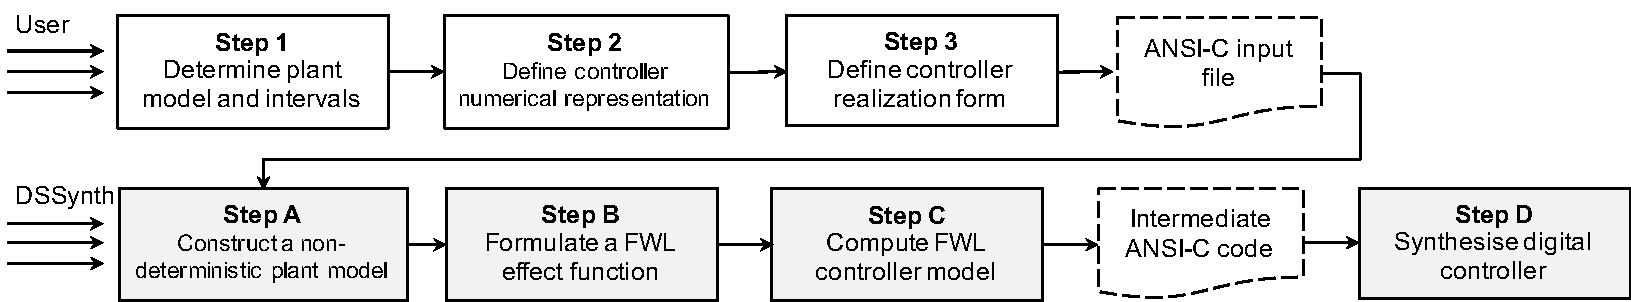
\includegraphics[width=0.9\textwidth]{figures/synthesis-flow.pdf}
\vspace{0.1cm}
\caption{Overview of the synthesis process\label{DSSynth_process}}
\end{figure*}

%In Step $1$, the user provides inputs $G(z)$ and $\Delta{G}(z)$
%%$\%$ ({\it i.e.}, $\Delta{G}(z)$ as a percentage of $G(z)$)
%, which contain the plant model and the
%interval, respectively.  In Step $2$, a digital controller must be designed
%with any preferred method, where $C(z)$ is obtained.  The controller
%numerical representation and realization form are chosen in Steps $3$ and
%$4$, respectively.  In Step $5$, the user finally configures the
%verification parameters ({\it e.g.}, verification time, properties, and BMC
%tool).  After that, DSVerifier verification engine performs an (automatic)
%verification of the desired property $\phi$ ({\it i.e.}, stability).  The
%user steps described in Steps $1$--$5$ result in an ANSI-C code that should
%be used as an input for DSVerifier.

Given a plant model in ANSI-C syntax as input (Steps 1--3), \tool
constructs a non-deterministic model to represent the plant family,
i.e., it addresses plant variations as interval sets (Step~A),
and formulates a function (Step~B) using implementation details provided in
Steps~$2$ and $3$ to calculate the controller parameters to be
synthesized (Step~C).  Note that \tool synthesizes the controller 
coefficients for the given implementation aspects, i.e., numerical
representation and realization form.  Finally, \tool builds an intermediate 
ANSI-C code for the digital system implementation, which is used as input 
for the CEGIS engine (Step~D).

This intermediate ANSI-C code model contains a specification $\phi$ for the
property of interest (i.e., robust stability) and is passed to the
Counterexample-Guided Inductive Synthesis (CEGIS) module of
CBMC~\cite{ClarkeKL04}, where the controller is marked as the input variable
to synthesize.  CEGIS employs an iterative, counterexample-guided refinement
process, which is explained in detail in Section~\ref{synthesizer-general}. 
CEGIS reports a successful synthesis result if it generates a controller
that is safe with respect to~$\phi$.  In particular, the ANSI-C code model
guarantees that a synthesized solution is complete and sound with respect to
the stability property~$\phi$, since it does not depend on system inputs and
outputs.  In the case of stability, the specification~$\phi$ consists of a
number of assumptions on the polynomial coefficients, following Jury's
Criteria, as well as the restrictions on the representation of these
coefficients as discussed in detail in Section~\ref{synthesis-elements}.

% by the function $f$ (cf.~Eq.~\eqref{FWL_tf})
%In Step A, DSVerifier constructs a non-deterministic model to represent the
%plant family $\mathfrak{G}$ using $g_0$ and $\Delta{g}\%$, which are
%provided in Step $1$.  DSVerifier then formulates $\mathcal{F}\langle I,F \rangle(\cdot)$ in
%Step B using implementation details provided from Steps $2$ and $3$, and
%then computes $\mathcal{F}\langle I,F \rangle(c_0)$ in Step C.  Thus, DSVerifier builds an
%intermediate ANSI-C code for the digital system implementation, which is
%used as input for the model-checker, as pointed in Step D.

%This intermediate ANSI-C code model has three main modules: digital
%controller code to be embedded into the microprocessor; plant model code,
%which simulates the plant model dynamics considering uncertainties; and
%``assert'' and ``assume'' statements, which control the verification flow. 
%For the digital controller code, transfer functions coefficients are
%quantised and deterministic, and all operations use fixed-point arithmetic. 
%\textcolor{red}{In the plant model code, transfer function coefficients are
%not quantised, but represented with maximum precision based on float
%data-type variables}; they are treated as non-deterministic variables to
%support model uncertainties.  The directive ``assume'' bounds
%non-deterministic variables, {\it i.e.}, inputs and plant uncertain
%coefficients.
%
%The translation of ANSI-C code into SAT/SMT formulae
%is done by a back-end model-checking tool ({\it e.g.},
%CBMC~\cite{ClarkeKL04} or ESBMC~\cite{CordeiroFM12}).  Here, DSVerifier
%symbolically checks a given property $\phi$ with respect to closed-loop
%systems, which are composed by $f(c_i)$ and every $G$ in $\mathfrak{G}$. 
%If any property violation is found, then DSVerifier reports a
%counterexample, which contains system inputs or parametric deviations
%$\Delta{G}$ that lead the system to a failure.  A successful verification
%result is reported if the system is safe with respect to $\phi$.  In
%particular, the stability verification is complete and sound, since it does
%not depend on system outputs and inputs.

%%%%%%%%%%%%%%%%%%%%%%%%%%%%%%%%%%%%%%%%%%%%%%%%%%%%%%%%%%%%%%%%%%%%%%%%%%%%%%%%%%%%%%
%\section{Modelling Errors} 

%In this section, we show how to embed discretization errors on the plant model, as follows: 
%%$\hat{G}(z)$ is split into two terms:
%%
%\begin{equation}
%\label{eq:uncertainplant}
%%\hat{G}(z)=G(z)+\Delta{G(z)},
%\tilde G(z) = \hat G(z) + \Delta G_P(z) = G(z,T) + \Delta G_Q(z) + \Delta G_P(z),   
%\end{equation}
%where $G(z,T)$ is the time discretization of the nominal physical plant $G(s)$, 
%$\Delta{G_{Q}(z)}$ represents the quantization uncertainty model, 
%and $\Delta{G_{P}(z)}$ describes the parametric uncertainty model. 

%\noindent where $G(z)$ is the discretised nominal plant model and
%$\Delta{G(z)}$ is the additive uncertainty, which is related to parametric
%uncertainties~\cite{Bessa16}.  

%\section{An Uncertainty Model for the quantization Error} 
%\label{sec:uncertainty-model-quantization-error}
%
%%Here, an uncertainty model to accommodate the
%%quantization noise effects on $\hat{G}(z)$ is proposed.  
%%As a result, Eq.~\eqref{eq:uncertainplant} is rewritten as
%%
%%\begin{equation}
%%\label{eq:uncertainFWLplant}
%%\hat{G}(z)=G(z)+\Delta{G_{Q}(z)}+\Delta{G_{P}(z)},
%%\end{equation}
%
%A model for $\Delta{G_{Q}(z)}$ that can represent the quantization
%noise effect in the plant output, and consequently the closed-loop system
%output, is proposed.  
%%\red{[eliminate next:] 
%%For convenience, the parametric uncertainties will be described here.}
%
%Consider the closed-loop sampled system in Figure~\ref{fig:sampledsystem},
%where $C(z)$ is the digital controller model, whose control output signal is
%quantised ($Q2$) and interpolated via a ZOH using digital-to-analog
%converter (DAC).  The quantization occurs because the DAC resolution may be
%different from the fixed point representation of the controller.  $G(s)$ is
%the continuous-time model of the plant, from which output samples are taken
%and quantised ($Q1$) by means of an analog-to-digital converter (ADC)
%synchronized with the DAC.  Each quantiser ($Q1$ and $Q2$) will present some
%contribution for the total quantization noise.
%    
%\begin{figure*}[ht]
%\centering
%
%\tikzset{add/.style n args={4}{
%    minimum width=6mm,
%    path picture={
%        \draw[circle] 
%            (path picture bounding box.south east) -- (path picture bounding box.north west)
%            (path picture bounding box.south west) -- (path picture bounding box.north east);
%        \node[draw=none] at ($(path picture bounding box.south)+(0,0.13)$)     {\small #1};
%        \node[draw=none] at ($(path picture bounding box.west)+(0.13,0)$)      {\small #2};
%        \node[draw=none] at ($(path picture bounding box.north)+(0,-0.13)$)    {\small #3};
%        \node[draw=none] at ($(path picture bounding box.east)+(-0.13,0)$)     {\small #4};
%        }
%    }
% }
%
%\resizebox{.8\textwidth}{!}{
% \begin{tikzpicture}[scale=0.6,-,>=stealth',shorten >=.2pt,auto,
%     semithick, initial text=, ampersand replacement=\&,]
%
%  \matrix[nodes={draw, fill=none, shape=rectangle, minimum height=.2cm, minimum width=.2cm, align=center}, row sep=.6cm, column sep=.3cm] {
%    \node[draw=none] (r) {$\tilde R(z)$};
%%   \& \coordinate (aux0);
%   \& \node[circle,add={-}{+}{}{}] (circle) {};
%   \node[draw=none] (ez) at ([xshift=1cm,yshift=.15cm]circle)  {$\tilde e(z)$};
%   \& \node[rectangle,draw,
%	minimum width=1cm,
%	minimum height=1cm,
%        label=\textbf{Controller}] (cz) {{\sc C(z)}};
%   \node[draw=none] (ud) at ([xshift=1cm,yshift=.15cm]cz)  {$\tilde U(z)$};
%     
%   \& complexnode/.pic={ 
%      \node[rectangle,draw,
%	minimum width=3cm,
%	minimum height=1.6cm,
%	label=\textbf{DAC},] (dac) {};
%     \node[circle,add={}{+}{+}{},fill=yellow!20] (q2) at ([xshift=-.65cm]dac.center) {};
%     \node[draw=none] (q2t)  at ([xshift=-.65cm,yshift=-.65cm]dac.center) {{\sc Q2}};
%     \node[draw=none] (v2)  at ([xshift=-.65cm,yshift=1.5cm]dac.center) {$\nu_2(z)$};
%     \node[fill=yellow!20] (zoh) at ([xshift=.65cm]dac.center) {{\sc ZOH}};}
%   \& \node[rectangle,draw,
%	minimum width=1cm,
%	minimum height=1cm,
%        label=\textbf{Plant}] (gs) {{\sc G(s)}};
%   \node[draw=none] (ud) at ([xshift=-1cm,yshift=.15cm]gs)  {$U(s)$};
%   \node[draw=none] (y) at ([xshift=1cm,yshift=.15cm]gs)  {$Y(s)$};
%   \& complexnode/.pic={ 
%     \node[rectangle,draw,
%	minimum width=4cm,
%	minimum height=1.6cm,
%	label=\textbf{ADC},] (adc) {};
%   \draw[] ([xshift=-1cm]adc.center) -- ++(0.5,0.2cm);
%   \coordinate (switch1) at ([xshift=-1cm]adc.center);
%   \coordinate (switch2) at ([xshift=-0.4cm]adc.center);
%   \node[circle,add={}{+}{+}{},fill=yellow!20] (q1) at ([xshift=1cm]adc.center) {};} 
%     \node[draw=none] (q2t)  at ([xshift=1cm,yshift=-.65cm]adc.center) {{\sc Q1}};
%   \node[draw=none] (v1)  at ([xshift=1cm,yshift=1.5cm]adc.center) {$\nu_1(z)$};
%   \& \coordinate (aux1);
%   \& \node[draw=none] (yz) {$\tilde Y(z)$};\\
%   \& \coordinate (aux3); 
%   \&
%   \&
%   \& 
%   \& 
%   \& \coordinate (aux2);\\
%  };
%
%
%  \path[->] (v1) edge (q1.north);
%  \path[->] (v2) edge (q2.north);
%  \path[->] (r) edge (circle.west);
%  \path[->] (aux1) edge (yz);
%  \path  
%   (circle.east) edge (cz)
%   (cz.east) edge (q2.west)
%   (q2.east) edge (zoh.west)
%   (zoh.east) edge (gs.west)
%   (switch2) edge (q1.west)
%   (q1.east) edge (aux1.west)
%   (gs.east) edge (switch1.west)
%   (aux1.south) edge (aux2.north)
%   (aux2.west) edge (aux3.east); 
%  \path[->]  (aux3.north) edge (circle.south);
% \end{tikzpicture}
%}
% \caption{Sampled System. \label{fig:sampledsystem}}
%\end{figure*}
%
%%% \begin{figure}[ht]
%%% \centering
%%% 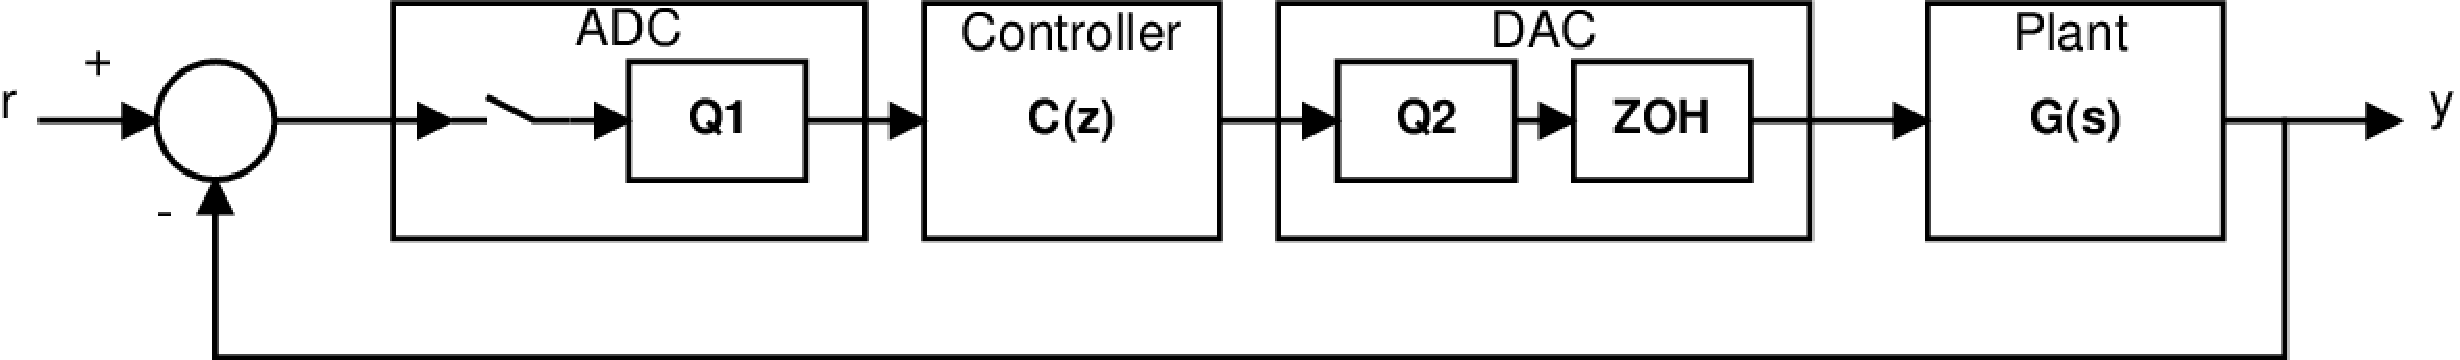
\includegraphics[width=\columnwidth]{figures/hsystembd.pdf}
%%% \caption{Sampled system.}
%%% \label{fig:sampledsystem}
%%% \end{figure}
%
%
%\begin{figure}[ht]
%\centering
%
%\tikzset{add/.style n args={4}{
%    minimum width=6mm,
%    path picture={
%        \draw[circle] 
%            (path picture bounding box.south east) -- (path picture bounding box.north west)
%            (path picture bounding box.south west) -- (path picture bounding box.north east);
%        \node[draw=none] at ($(path picture bounding box.south)+(0,0.13)$)     {\small #1};
%        \node[draw=none] at ($(path picture bounding box.west)+(0.13,0)$)      {\small #2};
%        \node[draw=none] at ($(path picture bounding box.north)+(0,-0.13)$)    {\small #3};
%        \node[draw=none] at ($(path picture bounding box.east)+(-0.13,0)$)     {\small #4};
%        }
%    }
% }
%
%\resizebox{.5\textwidth}{!}{
% \begin{tikzpicture}[scale=0.3,-,>=stealth',shorten >=.2pt,auto,
%     semithick, initial text=, ampersand replacement=\&,]
%
%  \matrix[nodes={draw, fill=none, shape=rectangle, minimum height=.2cm, minimum width=.2cm, align=center}, row sep=.6cm, column sep=.3cm] {
%    \node[draw=none] (r) {$R(z)$};
%%   \& \coordinate (aux0);
%   \& \node[circle,add={-}{+}{}{}] (circle) {};
%   \node[draw=none] (ez) at ([xshift=1cm,yshift=.15cm]circle)  {$e(z)$};
%   \& \node[rectangle,draw,
%	minimum width=1cm,
%	minimum height=1cm,
%        label=\textbf{Controller}] (cz) {{\sc C(z)}};
%   \node[draw=none] (ud) at ([xshift=1cm,yshift=.15cm]cz)  {$U(z)$};
%   \& \node[rectangle,draw,
%	minimum width=1cm,
%	minimum height=1cm,
%        label=\textbf{Plant}] (gs) {{\sc G(z)}};
%   \node[draw=none] (y) at ([xshift=1cm,yshift=.15cm]gs)  {$Y(z)$};
%
%   \& \node[circle,add={}{+}{+}{}] (circle2) {};
%%   \node[draw=none] (tyz) at ([xshift=-1cm,yshift=.15cm]circle2)  {$Y(z)$};
%   \node[draw=none] (nu) at ([yshift=1cm]circle2)  {$\nu(z)$};
%   \& \coordinate (aux1);
%   \& \node[draw=none] (yz) {$\tilde Y(z)$};\\
%   \& \coordinate (aux3); 
%   \&
%   \& 
%   \& 
%   \& \coordinate (aux2);\\
%  };
%
%
%%  \path[->] (v1) edge (q1.north);
%%  \path[->] (v2) edge (q2.north);
%  \path[->] (r) edge (circle.west);
%  \path[->] (nu) edge (circle2.north);
%  \path[->] (aux1) edge (yz);
%  \path  
%   (circle.east) edge (cz)
%   (cz.east) edge (gs.west)
%   (gs.east) edge (circle2.west)
%   (circle2.east) edge (aux1.west)
%   (aux1.south) edge (aux2.north)
%   (aux2.west) edge (aux3.east); 
%  \path[->]  (aux3.north) edge (circle.south);
% \end{tikzpicture}
%}
% \caption{Sampled System. \label{fig:sampledsystem}}
%\end{figure}
%
%%
%%
%
%\begin{figure}[ht]
%\centering
%
%\tikzset{add/.style n args={4}{
%    minimum width=6mm,
%    path picture={
%        \draw[circle] 
%            (path picture bounding box.south east) -- (path picture bounding box.north west)
%            (path picture bounding box.south west) -- (path picture bounding box.north east);
%        \node[draw=none] at ($(path picture bounding box.south)+(0,0.13)$)     {\small #1};
%        \node[draw=none] at ($(path picture bounding box.west)+(0.13,0)$)      {\small #2};
%        \node[draw=none] at ($(path picture bounding box.north)+(0,-0.13)$)    {\small #3};
%        \node[draw=none] at ($(path picture bounding box.east)+(-0.13,0)$)     {\small #4};
%        }
%    }
% }
%
%\resizebox{.5\textwidth}{!}{
% \begin{tikzpicture}[scale=0.3,-,>=stealth',shorten >=.2pt,auto,
%     semithick, initial text=, ampersand replacement=\&,]
%
%  \matrix[nodes={draw, fill=none, shape=rectangle, minimum height=.2cm, minimum width=.2cm, align=center}, row sep=.6cm, column sep=.3cm] {
%    \node[draw=none] (r) {$R(z)$};
%%   \& \coordinate (aux0);
%   \& \node[circle,add={-}{+}{}{}] (circle) {};
%   \node[draw=none] (ez) at ([xshift=1cm,yshift=.15cm]circle)  {$e(z)$};
%   \& \coordinate (aux4);
%   \& \node[rectangle,draw,
%	minimum width=1cm,
%	minimum height=1cm,
%        label=\textbf{Controller}] (cz) {{\sc C(z)}};
%   \node[draw=none] (ud) at ([xshift=1cm,yshift=.15cm]cz)  {$U(z)$};
%   \& \node[rectangle,draw,
%	minimum width=1cm,
%	minimum height=1cm,
%        label=\textbf{Plant}] (gs) {{\sc G(z)}};
%   \node[draw=none] (y) at ([xshift=1cm,yshift=.15cm]gs)  {$Y(z)$};
%   \& \node[circle,add={+}{+}{}{}] (circle2) {};
%%   \node[draw=none] (tyz) at ([xshift=-1cm,yshift=.15cm]circle2)  {$Y(z)$};
%%   \node[draw=none] (nu) at ([yshift=1cm]circle2)  {$\nu(z)$};
%   \& \coordinate (aux1);
%   \& \node[draw=none] (yz) {$\tilde Y(z)$};\\
%   \& 
%   \& \coordinate (aux5); 
%   \& \node[rectangle,draw,
%	minimum width=1cm,
%	minimum height=1cm] (deltag) {{\sc $\Delta G(z)$}};
%   \&
%   \& \coordinate (aux6);\\
%   \& \coordinate (aux3); 
%   \&
%   \& 
%   \& 
%   \&
%   \& \coordinate (aux2);\\
%  };
%
%
%%  \path[->] (v1) edge (q1.north);
%%  \path[->] (v2) edge (q2.north);
%  \path[->] (r) edge (circle.west);
%%  \path[->] (nu) edge (circle2.north);
%  \path[->] (aux1) edge (yz);
%  \path  
%   (aux4.north) edge (aux5.south)
%   (aux5.east) edge (deltag.west)
%   (deltag.east) edge (aux6.west)
%   (aux6.south) edge (circle2.south)
%   (circle.east) edge (cz)
%   (cz.east) edge (gs.west)
%   (gs.east) edge (circle2.west)
%   (circle2.east) edge (aux1.west)
%   (aux1.south) edge (aux2.north)
%   (aux2.west) edge (aux3.east); 
%  \path[->]  (aux3.north) edge (circle.south);
% \end{tikzpicture}
%}
% \caption{Sampled System. \label{fig:sampledsystem}}
%\end{figure}




%\begin{myprop}
%Considering the quantization noise $\nu(k)$ as an output error in the
%discrete plant model, 
%%{\it i.e.}, it does not affect the plant dynamics, but its output samples, 
%$\Delta{G_{Q}(z)}$ can be obtained from
%%
%\begin{equation}
%\label{eq:quantization_tf}
%\Delta{G_{Q}(z)}=\frac{\nu(z)}{U(z)},
%\end{equation}
%where $\nu(z)$ is the z-transform of the random process $\nu(k)$,
%which can be calculated through the power spectral density of
%$\nu(k)$~\cite{poularikas2000transforms}.  
%Thus, the $\Delta{G_{Q}(z)}$ can expressed as
%%
%\begin{equation}
%\label{eq:deltag_var}
%\Delta{G_{Q}(z)}=\frac{\sigma_{Q}^{2}}{U(z)},
%\end{equation}
%where $\sigma_{Q}^{2}$ is the variance of the quantization noise and
%$U(z)$ is the z-transform of control signal ({\it i.e.}, the z-transform of
%the signal from the digital controller), which is provided to the plant by
%means of ZOH.
%\end{myprop}
%
%%
%\begin{proof}
%%
%Suppose that the plant discrete model in Figure~\ref{fig:sampledsystem} can
%be represented by the following pulse transfer function (without
%quantization noise effect):
%%
%\begin{equation}
%\label{eq:tfwithout}
%G(z)=\frac{Y(z)}{U(z)}=\frac{B(z)}{A(z)}=\frac{b_{0}+b_{1}z^{-1}+b_{2}z^{-2}+\cdots+b_{M}z^{-M}}{1+a_{1}z^{-1}+a_{2}z^{-2}+\cdots+a_{N}z^{-N}},
%\end{equation}
%%
%\noindent where $Y(z)$ is the z-transform of the plant output signal without
%noise $y(k)$, $U(z)$ is the z-transform of the control signal, which is
%provided to the plant, $A(z)$ and $B(z)$ are the plant pulse transfer
%function numerator and denominator, respectively.
%
%Considering the quantization noise $\nu(k)$ as an output error in the
%discrete plant model, an additive noise in the plant output $y(k)$ resulting
%in the noisy output $\hat{y}(k)$ can be represented as
%%
%\begin{equation}
%\hat{y}(k)=y(k)+\nu(k).
%\end{equation}
%
%Note that the model in Eq.~\eqref{eq:tfwithout} is equivalent to the
%following difference equation:
%%
%\begin{equation}
%\begin{split}
%y(k)=-a_{1}y(k-1)-a_{2}y(k-2)-\cdots - a_{N}y(k-N)\\
%+b_{0}u(k)+b_{1}u(k-1)+b_{2}u(k-2)+\cdots+b_{M}u(k-M),
%\end{split}
%\end{equation}
%
%\noindent and consequently $\hat{y}(k)$ can be represented by the following
%difference equation:
%%
%\begin{equation}
%\label{eq:differencewithnoise}
%\begin{split}
%\hat{y}(k)=-a_{1}y(k-1)-a_{2}y(k-2)-\cdots - a_{N}y(k-N)\\
%+b_{0}u(k)+b_{1}u(k-1)+b_{2}u(k-2)+\cdots+b_{M}u(k-M)+\nu(k).
%\end{split}
%\end{equation}
%
%The z-transform of Eq.~\eqref{eq:differencewithnoise} is
%%
%\begin{equation}
%\begin{split}
%\hat{Y}(z)=(-a_{1}z^{-1}-a_{2}z^{-2}-\cdots-a_{N}z^{-N})Y(z)\\
%+(b_{0}+b_{1}z^{-1}+b_{2}z^{-2}+\cdots+b_{M}z^{-M})U(z)+\nu(z),
%\end{split}
%\end{equation}
%dividing both sides by $U(z)$, it is equivalent to:
%\begin{equation}
%\frac{\hat{Y}(z)}{U(z)}=\hat{G}(z)=[1-A(z)]G(z)+U(z)B(z)+\frac{\nu(z)}{U(z)}.
%\end{equation}
%
%Considering $\hat{G}(z)=G(z)+\Delta{G_{Q}(z)}$ and Eq.~\eqref{eq:tfwithout},
%the intended expression can be obtained as
%%
%\begin{equation}
%\Delta{G_{Q}(z)}=\frac{\nu(z)}{U(z)} 
%\end{equation}
%\end{proof}

%Eq.~\eqref{eq:deltag_var} indicates that the modelling of the quantization noise
%effect on the plant transfer function demands an estimation of the variance
%of quantization noise $\sigma_{Q}^{2}$.  To obtain such estimation, the
%methodology presented by~\cite{widrow2008quantization}
%is used.  The authors provide an algorithm for computing the mean square of
%the output noise due to $Q1$ and $Q2$.  Considering that each quantiser
%contribution can be represented by a white noise with zero mean
%(Assumption~\ref{whitenoise}), the mean square can be considered as the
%variance of noise ($\sigma_{Q}^{2}$), which can be calculated as
%%
%\begin{equation}
%\sigma_{Q}^{2}=\frac{\lambda_{1}^{2}\cdot \sum {h_{Q1}^{2}} \cdot q_{1}+\lambda_{2}^{2}\cdot \sum {h_{Q2}^{2}} \cdot q_{2}}{12},
%\end{equation}
%%
%\noindent where $\lambda_{1}$ and $\lambda_{2}$ are the scale factors, {\it i.e.} constant gains usually employed before the ADC and after the DAC in order to avoid the overload of converters  %\red{[define scale factors]} 
%for the quantization $Q1$ and $Q2$, respectively; $q_{1}$ and $q_{2}$ are the quantization step for $Q1$ and $Q2$, respectively, and $\sum {h_{Q1}^{2}}$ and $\sum
%{h_{Q2}^{2}}$ are the squares sums of the impulse response obtained by means
%of a transfer function from $Q1$ and $Q2$ to the plant output, respectively.
%
%The transfer functions $H_{Q1}(z)$ and $H_{Q2}(z)$, from which the squares
%sums of the impulse response are needed, can be obtained through the
%analysis of the system in Figure~\ref{fig:sampledsystem}. 

%\red{[The following text needs to be completed. (Notice typos, reference to wrong signal $R$, and to wrong TF $C,G$.]}
%
%Considering that
%the quantiser $Q1$ is the source of a white noise with zero mean $\nu_{1}$
%and $Q2$ is the source of a white noise with zero mean $\nu_{2}$, the
%following equation can be written for the system in
%Figure~\ref{fig:sampledsystem}
%%
%\begin{equation}
%\resizebox{0.48\textwidth}{!}{
%$\tilde{Y}(z)=\tilde R(z)C(z)G(z)-\tilde{Y}(z)C(z)G(z)+\nu_{1}(z)+\nu_{2}(z)G(z),$
%}
%\end{equation}
%
%\noindent which can be rewritten as
%%
%\begin{equation}
%\label{eq:outputfunctions}
%\tilde{Y}(z)=C(z)G(z)H(z)R(z)+H(z)\nu_{1}(z)+G(z)H(z)\nu_{2}(z)
%\end{equation}
%$$H(z)=\frac{1}{1+C(z)G(z)}$$
%
%Note that $H(z)$ cancels the poles of both $G(z)$ and $C(z)$, thus we need only verify the stability of $H(z)$
%to validate the stability of the whole system.
%These equations are sufficient for computing $\sigma_{Q}^{2}$.  However,
%there is still a gap for a complete model for $\Delta{G_{Q}(z)}$ in
%Eq.~\eqref{eq:deltag_var}, {\it i.e.}, the z-transform of control action
%$U(z)$.  This indicates that the quantization noise effect on a discrete
%plant model mainly depends on three main factors:
%%
%\begin{itemize}
%%
%\item \textbf{Sample time:} the sample time effect is reflected over pulse transfer function that covers the effects of DAC ant its interpolator (ZOH) \red{[clarify/revise based on the comments made above.]};
%%
%\item \textbf{ADC and DAC step:} \red{[again, do we need both?]} these are the main component of quantization noise power, but an $8$-bits converter already reduces the effect of quantization noises in the output for negligible values.
%%
%\item \textbf{Signal-to-noise ratio (SNR): } the dependence on the value of $U(z)$ \red{[notice that now we have reduced the problem to depend on the effect of the reference signal transform R(z) - pls revise.]} shows the importance of the SNR for handling quantization noise; for a high SNR of the digital controller, the quantization effect is negligible. This happens during the transient of the system, when high control actions are employed. However, it can be relevant during the steady state. A digital controller with integral action might be sufficient for eliminating such influence at steady state.
%%
%\end{itemize}
%
%An alternative expression for $\Delta{G_{Q}(z)}$ can be obtained from
%Eq.~\eqref{eq:deltag_var}, transforming it into a function of the reference
%$R(z)$.  Once $U(z)$ is the control signal obtained via digital controller
%$C(z)$ and error signal, {\it i.e.},
%%
%\begin{equation}
%U(z)=C(z)\cdot[R(z)-Y(z)],
%\end{equation} 
%
%\noindent where $Y(z)$ is the first term of Eq.~\eqref{eq:outputfunctions}, thus:
%\begin{equation}
%\label{eq:controlsignal}
%\resizebox{0.48\textwidth}{!}{
%$U(z)=C(z)\cdot \left[R(z)-\frac{C(z)G(z)}{1+C(z)G(z)}R(z)\right]=\frac{C(z)}{1+C(z)G(z)}R(z).$
%}
%\end{equation} 
%
%Substituting Eq.~\eqref{eq:controlsignal} in Eq.~\eqref{eq:deltag_var}, a
%model for $\Delta{G_{Q}(z)}$ depending on $R(z)$ can be obtained:
%%
%\begin{equation}
%\Delta{G_{Q}(z)}=\sigma^{2}_{Q}\cdot \frac{1+C(z)G(z)}{C(z)} \cdot \frac{1}{R(z)},
%\end{equation}
%
%\noindent where $R(z)$ can be considered as a step signal (for stabilization
%purpose) with height equal to $r$, which can be rewritten as
%%
%\begin{equation}
%\Delta{G_{Q}(z)}=\frac{\sigma^{2}_{Q}}{r}\cdot \frac{1+C(z)G(z)}{C(z)} \cdot \frac{z-1}{z}.
%\end{equation}
%
%A more precise description of $\Delta{G_{Q}(z)}$ can be obtained
%considering FWL \red{[clarify what you mean with FWL, introduce FWL function explicitly and precisely]} effects on digital controller coefficients, as described in
%Bessa {\it et al.}~\cite{Bessa16}, {\it i.e.}, using $FWL[C(z)]$ instead of
%the nominal $C(z)$:
%%
%\begin{equation}
%\label{eq:deltaG_final}
%\Delta{G_{Q}(z)}=\frac{\sigma^{2}_{Q}}{r}\cdot \frac{1+FWL[C(z)]G(z)}{FWL[C(z)]} \cdot \frac{z-1}{z}.
%\end{equation}
%
%Finally, Eq.~\eqref{eq:deltaG_final} is a suitable frequency domain model
%for quantization noise effects on closed-loop systems.  This model depends
%on the plant pulse transfer function ($G(z)$), which is described by
%Eq.~\eqref{eq:pulsetf}, the height of step reference signal $r$, and the
%digital controller model.

%\subsection{Modelling Error on Parameters Representation} 
%\label{sec:}

%\red{[TO BE COMPLETED.]}
% We use CounterExample-Guided Inductive Synthesis (CEGIS), as
% illustrated in Fig~\ref{fig:CEGIS}.

%specialised it for stream refactoring.  
% adding JST for stream refactoring

\subsection{Architecture of the Program Synthesizer}
\label{synthesizer-general}
%
%% \red{[I would recommend to clarify the domain of definition of $\sigma$, particularly over the set where $x$ ranges over. 
%% (Be cognisant that control audience might be unfamiliar with the cegis architecture.) ]}
% 
The input specification provided to the program synthesizer is of the form
$\exists \vec{P} .  \forall \vec{x}.  \sigma(\vec{x}, \vec{P})$ where
$\vec{P}$ ranges over functions, $\vec{x}$ ranges over ground terms and
$\sigma$ is a quantifier-free formula.  We interpret the ground terms over
some finite domain $\mathcal{D}$.

The design of our synthesizer is given in Figure~\ref{fig:CEGIS} and consists
of two phases, {\sc Synthesize} and {\sc Verify}, which interact via a
finite set of test vectors {\sc inputs} that is updated incrementally. 
Given the aforementioned specification $\sigma$, the {\sc synth} procedure
tries to find an existential witness $\vec{P}$ satisfying the specification
$\sigma(\vec{x}, \vec{P})$ for all $\vec{x}$ in {\sc inputs} (as opposed to
all $\vec{x} \in \mathcal{D}$).
%
If {\sc synthesize} succeeds in finding a witness~$\vec{P}$, this witness
is a candidate solution to the full synthesis formula.  We pass this
candidate solution to {\sc verify}, which checks whether it is a full
solution (i.e., $\vec{P}$ satisfies the specification $\sigma(\vec{x},
\vec{P})$ for all $\vec{x}\in\mathcal{D}$).
%
%determines whether
%it does satisfy the specification on all inputs by checking
%satisfiability of the following verification formula:
%
%$\exists \vec{x} . \lnot \sigma(\vec{x}, \vec{P})$
%If this formula is unsatisfiable, 
%% the candidate solution is in fact a 
%% full solution.
%
If this is the case, then the algorithm terminates.  Otherwise, additional
information is provided to the {\sc synthesize} phase in the form of a new
counterexample that is added to the {\sc inputs} set and the loop iterates
again (note that, for now, we ignore the second feedback signal ``Increase
Precision'' provided by the {\sc Verify} phase in Figure~\ref{fig:CEGIS} as it
is specific to control synthesis and will be described in the next section).

%% the witness $\vec{x}$ denote an input on which the
%% candidate solution fails to meet the specification.  Thus, $\vec{x}$ is
%% added to the {\sc inputs} set, and the loop iterates again.  

It is worth noting that each iteration of the loop adds a new input to
the finite set $\text{\sc inputs}$ that is used for synthesis.  Given
that the full set of inputs $\mathcal{D}$ is finite, this means that
the refinement loop can only iterate a potentially very large, but
finite number of times.

\subsection{Synthesis for Control}
\label{synthesis-elements}

\paragraph{Formal specification of the stability property}

Next, we describe the specific property that we pass to the program
synthesizer as the specification $\sigma$.  There are a number of 
algorithms in our verification engine that can be used for stability analysis~\cite{daes20161, Bessa16}.  
%one based on Schur's decomposition
%and another one based on Jury's criterion~\cite{astrom1997computer}.  
Here we choose Jury's criterion~\cite{astrom1997computer} in view of its efficiency \blue{[check correctness] and ease of integration within \tool}: 
we employ this method to check the stability in the $z$-domain for the
characteristic polynomial $S(z)$ defined in~\eqref{eq:internal_stab_lemma}.
%
% of the matrix $\left( \begin{array}{c} Y \\ U \end{array}\right)$, where $Y(z)$ is the closed-loop system output and U(z) is the controller output. 
%% \red{[unclear: what matrix? We need to clarify the relationship
%% between the char. poly. $S(z)$ and the later quantities $\Delta
%% N_{G}(z), \Delta D_{G}(z)$ and corresponding controller's
%% structure.]}.
%
We~consider the following form for $S(z)$:
%
\begin{equation*}
S(z) = a_0z^N+a_1z^{N-1}+\cdots+a_{N-1}z+a_N=0, a_0\neq0. 
\end{equation*}
%\cdsay{is this for the matrix $\left( \begin{array}{c} Y \\ U \end{array}\right)$?}

% Assuming that $\hat{G}(z) = \frac{\hat{N_G}(z)}{\hat{D_G}(z)}$
% and $\hat{C}(z) = \frac{\hat{N_C}(z)}{\hat{D_C}(z)}$, then:
% $$S(z) = FWL[N_C(z)] \times \hat{N_G}(z) + FWL[D_C(z)] \times \hat{D_G}(z)$$
Next, the following matrix
$M = [m_{ij}]_{(2N-2)\times N}$ is built from $S(z)$ coefficients:
%
$$
M=\left( 
\begin{array}{c}
V^{(0)}\\
V^{(1)}\\
\vdots\\
V^{(N-2)}
\end{array}
\right), 
$$
%
where $V^{(k)} = [v^{(k)}_{ij} ]_{2\times N}$ such that:
%
$$
v_{ij}^{(0)}=\left\{
\begin{array}{ll}
a_{j-1}, & \texttt{if}~i=1\\
v_{(1)(N-j+1)}^{0},&\texttt{if}~i=2
\end{array}
\right.
$$
%
$$
v_{ij}^{(k)}=\left\{
\begin{array}{ll}
0,&\texttt{if}~j>n-k\\
v_{1j}^{(k-1)}-v_{2j}^{(k-1)} . \frac{v_{11}^{(k-1)}}{v_{21}^{(k-1)}}, & \texttt{if}~j\leq n-k ~\texttt{and}~i=1\\
v_{(1)(N-j+1)}^{k},& \texttt{if}~j\leq n-k ~\texttt{and}~i=2\\
\end{array}
\right.
$$
%
and where $k \in \mathbb{Z}$ is such that $0 < k < N - 2$. 
We have that~\cite{astrom1997computer} 
$S(z)$ is the
characteristic polynomial of a stable system if and only if the following four conditions hold:
%\begin{itemize}
%\item 
$R_1: S(1) > 0$;
%\item 
$R_2: (−1)^N S(−1) > 0$;
%\item 
$R_3: |a_0| < a_N$;
%\item 
$R_4: m_{11} > 0 \wedge\allowbreak
      m_{31}>0 \wedge\allowbreak
      m_{51}>0 \wedge \ldots \wedge\allowbreak
      m_{(2N{-}3)(1)}>0$.
%\end{itemize}
%
The stability property is then encoded by a constraint of the form:
$
\phi_\mathit{stability} \equiv (R_1 \wedge R_2 \wedge R_3 \wedge R_4).
$
%\cdsay{figure out what is existentially quantified for the final $\sigma$.} 
%% \red{[Yes, intuitively all clear, however for the sake of clarity I would like to see the explicit mapping between the above formula and the previously used specification 
%% $\sigma(x, P)$, with clear elucidation of the relationship between the domain of $z$ and that of $x$.]}

% \red{[clear elucidation of the mapping between this and the domains used 
% in the general description of the synthesiser]}

\paragraph{The synthesis problem}
The synthesis problem we are trying to solve is the following:
find a digital controller $\tilde C(z)$ %denoted by  $N_c$ and $D_c$ 
that makes the closed-loop system stable 
for all possible uncertainties 
%$\Delta{\vec{p}}$ (\ref{eq:uncertainty}).
$\tilde G(z)$ \eqref{digital_plant_tf}.
%, where we precisely describe 
%$(\Delta N_G, \Delta D_G)$. 
% Note that, similar to the rest of the paper, we use the notation 
% $\tilda{N_G}(z) = N_G(z) + \Delta N_G(z)$ and 
% $\hat{N_C}(z) = N_C(z) + \Delta N_C(z)$.
When mapping back to the notation used for describing the general architecture 
of the program synthesizer, the controller $\tilde C(z)$ denotes $P$ and 
$\tilde G(z)$ represents $x$. 

As mentioned above, we compute the coefficients for $\tilde C(z)$ 
%$N_c$ and $D_c$ 
in the domain $\mathbb{R}\param{I}{F}$, 
%and $\mathbb{R}^{m_C}\param{I}{F}$, respectively, 
%where $n_C$ and $m_C$ denote the order of the corresponding polynomials
and those for $\tilde G(z)$ in the domain
$\mathbb{R}\langle I_p,F_p \rangle$.
While the controller's precision $\param{I}{F}$ is given, 
we can vary $\param{I_p}{F_p}$ such that 
$\mathbb{R}\langle I_p,F_p \rangle \supseteq \mathbb{R}\langle I,F \rangle$.
%
As the cost of SAT solving increases with in the size of the problem
instance, our algorithm tries to solve the problem first for small $I_p$,
$F_p$, iteratively increasing the precision if it is insufficient.

\subsection{The {\sc Synthesize} and {\sc Verify} phases}

The {\sc synthesize} phase uses BMC to 
compute a solution $\tilde C(z)$.
There are two approaches for the {\sc verify} phase.
The first approach uses interval arithmetic \cite{moore1966interval}
to represent the coefficients
$[{c}_i-\Delta_p{c}_i-\Delta_b{c}_i,\,\allowbreak
{c}_i+\Delta_p{c}_i-\Delta_b{c}_i+(2^{-F_p})]$ 
and rounds operations outwards during calculations.  This effectively allows
us to simultaneously evaluate the whole collection of plants $\hat{G}(s)$ (\emph{ie} all concrete plants $G(s)$ in the range $G(s) \pm \Delta_pG(s)$)
plus the effects of numeric calculations in the engine.  Synthesized
controllers using this verifier will always be stable for all plants in the
family.
% and only generate counterexamples when the precision of the
%engine is insufficient (\emph{ie} no stable plant could be found). 
Our preliminary experiments showed that a synthesis approach
using this verification engine has poor performance and we
%Given the high computational cost of this
%approach, 
therefore designed a second approach, which we describe below.
Our experimental results described in Section~\ref{sec:experiments}
%try both approaches and provide the time for the fastest. 
show that the speedup yielded by the second approach 
is in most cases of at least two orders of magnitude. 

The second approach is illustrated in Figure~\ref{fig:CEGIS} and uses a
two-stage verification approach: the first stage performs potentially unsound
fixed-point operations assuming a plant precision \param{I_p}{F_p}, and the
second stage restores soundness by validating these operations using
interval arithmetic on the synthesized controller.
%
\begin{figure*}[htb]
\centering
%\resizebox{1\textwidth}{!}
{
 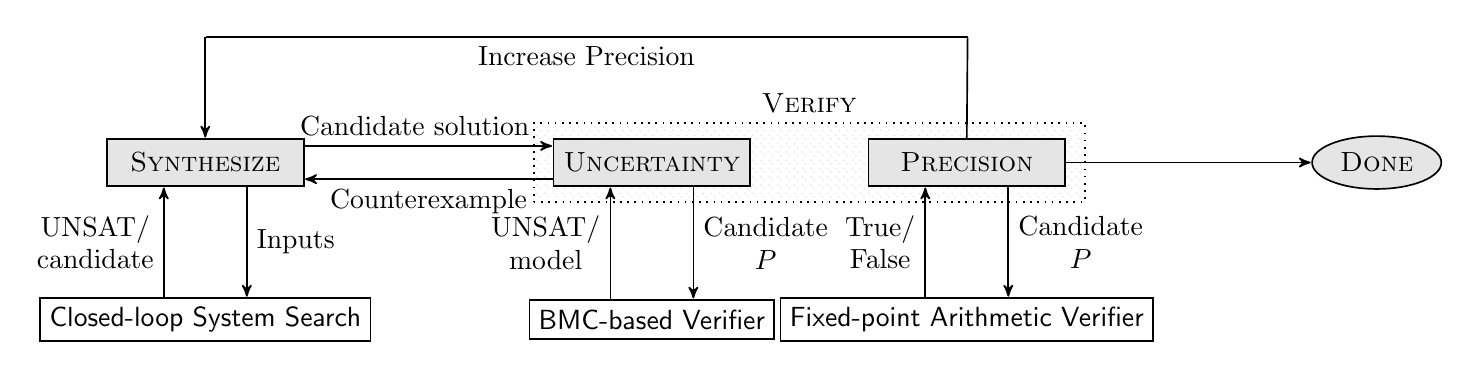
\begin{tikzpicture}[scale=0.3,->,>=stealth',shorten >=.2pt,auto, semithick, initial text=, ampersand replacement=\&,]
  \matrix[nodes={draw, fill=none, shape=rectangle, minimum height=.2cm, minimum width=.2cm, align=center
},
          row sep=.6cm, column sep=2cm] {
   \coordinate (aux1);
   \& \coordinate (aux2);
   \&;\\
   \node[minimum width=2.5cm, minimum height=0.6cm, fill=gray!20] (synth) {{\sc Synthesize}};
   \&
   complexnode/.pic={ 
     \node[rectangle,draw,dotted,
	minimum width=7cm,
	minimum height=1cm,
        pattern=north west lines, pattern color=gray!20,
	label={\sc Verify},] (verif) {};
     \node[minimum width=2.5cm, minimum height=0.6cm, fill=gray!20] (verif1) at ([xshift=-2cm]verif.center) {{\sc Uncertainty}};
     \node[minimum width=2.5cm, minimum height=0.6cm, fill=gray!20] (verif2) at ([xshift=2cm]verif.center) {{\sc Precision}};
   } 
   \& \node[ellipse, fill=gray!20] (done) {{\sc Done}};\\
   %% \node[fill=yellow!20] (verif) {{\sc ~~~~~~Uncertainty~~~~~~}};
   %% \&
   %% \node[fill=yellow!20] (verif2) {{\sc ~~~~~~Precision~~~~~~~}};\\
   \& \\
   \node[minimum height=0.5cm] (gp) {\sf Closed-loop System Search};
   \&
   complexnode/.pic={ 
     \coordinate (aux);
   \node[minimum height=0.5cm] (bmc) at ([xshift=-2cm]aux.center) {\sf BMC-based Verifier};
   \node[minimum height=0.5cm] (fp)  at ([xshift=2cm]aux.center) {\sf Fixed-point Arithmetic Verifier};
   }   
    \\
  };

   \path
    ([yshift=2em]synth.east) edge node[xshift=-0.5em] {Candidate solution} ([yshift=2em]verif1.west)
    ([yshift=-2em]verif1.west) edge node {Counterexample} ([yshift=-2em]synth.east)
    ([xshift=5em]verif1.south) edge node[align=center] {Candidate\\ $P$} ([xshift=5em]bmc.north)
    ([xshift=5em]verif2.south) edge node[align=center] {Candidate\\ $P$} ([xshift=5em]fp.north)
    ([xshift=-5em]bmc.north) edge node[align=center]  {UNSAT/\\model} ([xshift=-5em]verif1.south)
    ([xshift=-5em]fp.north) edge node[align=center]  {True/\\False} ([xshift=-5em]verif2.south)
    (verif2) edge node {} (done)
    ([xshift=5em]synth.south) edge node[align=center] {Inputs} ([xshift=5em]gp.north)
    ([xshift=-5em]gp.north) edge node[align=center] {UNSAT/\\candidate} ([xshift=-5em]synth.south)
    (aux1) edge (synth.north);
   \path[-]
   (verif2.north) edge node[align=center] {} ([xshift=6.7cm]aux2)
   ([xshift=6.7cm]aux2) edge node[align=center] {Increase Precision} (aux1);

 \end{tikzpicture}
}
\caption{Counterexample-Guided Inductive Synthesis of Closed-loop Systems (Step~D) in Figure~\ref{DSSynth_process}
\label{fig:CEGIS}}
\end{figure*}
%
%
In more detail, in the first stage, denoted by {\sc Uncertainty} in
Figure~\ref{fig:CEGIS}, assuming a precision \param{I_p}{F_p} we check
whether the system is unstable for the current candidate solution, i.e., if
$\neg \phi_\mathit{stability}$ is satisfiable for~$S(z)$.  If this is the
case, then we obtain a counterexample~$\tilde G(z)$,
%
%denoted by values for each coefficients of $\Delta N_{G}(z)$ and $\Delta D_{G}(z)$, 
%\red{[see my comment above - these quantities pop up too abruptly.]},
%
which makes the closed-loop system unstable.  This uncertainty is added to
the set {\sc inputs} such that, in the subsequent {\sc synthesize} phase, we
obtain a candidate solution consisting of a controller $C(z)$, which makes
the closed-loop system stable for all the uncertainties accumulated in {\sc
inputs}.

If the {\sc Uncertainty} verification stage concludes that the system is
stable for the current candidate solution, then we pass this solution to the
second verification stage, {\sc Precision}, which checks the propagation of
the error in the fixed-point calculations using a Fixed-point Arithmetic
Verifier based on interval arithmetic.
%
% To achieve this, we use a nondeterministic plant selected from $\mathfrak{G}(z)$ where the expected error of the bit vector calculations is assumed to be within the expected bounds and verified after synthesis using the interval version of the program. 
%
% The first verification phase produces a counterexample if some instance of $\mathfrak{G}(z)$ does not verify the properties and the CEGIS loop iteratively looks for a new controller that verifies the supplied counterexamples. The second phase verifies the propagation of the error in the fixed point calculations.
% If the second phase fails verification, we increase the precision of the analyser and feed the CEGIS loop again to find a sound solution. 
% vouches for the use of CEGIS in most of our benchmarks.
% \cdsay{end of integration}

If the {\sc precision} verification returns $\mathit{false}$, then we
increase the precision of \param{I_p}{F_p} and re-start the {\sc
  synthesize} phase with an empty {\sc inputs} set.  Otherwise, we
found a full sound solution for our synthesis problem and we are done.

In the rest of the paper, we will refer to the two approaches 
for the {\sc verify} phase as one-stage and two-stage, respectively.

%-----------------------------
\subsection{Soundness}
%-----------------------------

Within the scheme in Figure \ref{fig:CEGIS}, 
while the {\sc synthesise} phase searches for potentially unsound 
candidate solutions, the soundness of the model is ensured by the {\sc verify} phase.  
If a candidate solution is successfully verified, it is necessarily sound. 

Through its two stages, the {\sc verify} phase looks at two separate elements for
soundness.
% The first ensures that there exists no
% counterexample plant that would create a closed-loop with unstable
% poles. The fixed word length of the controller is not relevant at this
% point since the parameters have already been chosen to fit this
% criteria (i.e., the candidate solution is FWL).
The first stage ensures that no counterexample
plant with an unstable closed loop exists with % If no such
% system exists, then the controller is stable for all
% plants in the collection with
the limitations given by the data
type used by the verifier. Since the actual
plant works in the reals, whereas we use fixed/floating point
arithmetic to evaluate it, we need to ensure that the rounding errors
in the caculations do not cause the solution to be unsound.
% 
For this reason the second verification stage uses interval arithmetic with
outward rounding to ensure that these errors do not exceed critical
bounds that could make some plant unstable. 

This means that whilst the solution may not be complete, it is sound for
evaluating any collection of real plants with a defined FWL controller. 
We require two verification stages because,
while the second one can ensure the stability of all plants in the collection, 
it is unable to provide a counterexample.

%%%%%%%%%%%%%%%%%%%%%%%%%%%%%%%%%%%%%%%%%%%%%%%%%%%%%%%%%%%%%%%%%%%%%%%%%%%%%%%%%%%%%%
\subsection{Illustrative Example} \label{sec:running-ex}

We illustrate our approach with a classical cruise control example,
extracted from the literature~\cite{Astrom08}.  The example highlights the
challenges that arise when using finite-precision arithmetic in digital
control.  We are given a discrete plant model (with a time step of
$0.2$\,s), which is represented by the following $z$-expression:
%
\begin{equation}
\label{Eq:running-example-plant}
G(z) = \frac{0.0264}{z-0.9998}.
\end{equation}

Using an optimization tool, the authors
of~\cite{DBLP:conf/hybrid/WangGRJF16} have designed a high-performance
controller for this plant, which is characterized by the following
$z$-domain transfer function:
%
\begin{equation}
\label{Eq:running-example-controller}
C(z) = \frac{2.72z^2 - 4.153z + 1.896}{z^2 - 1.844z + 0.8496}.
\end{equation}
%
The authors of~\cite{DBLP:conf/hybrid/WangGRJF16} claim that the controller
$C(z)$ in~\eqref{Eq:running-example-controller} stabilizes the
closed-loop system for the discrete plant model $G(z)$ in~\eqref{Eq:running-example-plant}.  
However, if the effects of finite-precision arithmetic are considered (e.g., fixed-point arithmetic and
FWL), then this closed-loop system becomes unstable.
%
For instance, an implementation of $C(z)$ using 
$\mathbb R \param {4}{16}$ fixed-point
numbers (i.e., $4$ bits for the integer part and $16$ bits for the
fractional part) can be modeled as: 
%
\begin{equation}
\label{Eq:running-example-controller-quantized}
\resizebox{.47\textwidth}{!}{
$\tilde{C}(z) {:=} \frac{2.7199859619140625z^2{-}4.1529998779296875z
{+}1.89599609375}{z^2{-}1.843994140625z+0.8495941162109375}$. 
}
\end{equation} 
%
The resulting system using the typical series loop configuration, where
$\tilde{C}(z)$ and $G(z)$ are in the forward path, is unstable. 
\aabatecmt{[hang in there - did we not consider FWL on $G(z)$? why not?]}
\dariocmt{we are explaining the case where a real plant (no FWL) is not correctly stabilized by $\tilde{C}$, so although our analysis might evaluate $\tilde{G}(z)$, the problem statement is over $G(z)$}
Figure~\ref{fig:original} gives the Bode diagram for the digital controller
represented in~\eqref{Eq:running-example-controller}: 
as the phase margin is negative, 
the controller is unstable when considering the above FWL effects.

\subsection{Program Synthesis for the Example}
%
We now demonstrate how our approach solves the synthesis problem for the
example given in the previous section.  
Assuming a precision of $I_p=16$, $F_p=24$,  
we start with an a-priori candidate solution with all coefficients zero (note that the controller is in the FWL domain, hence we use $\tilde{C}(z)$): 
%
$$ 
\tilde{C}(z)=\frac{0z^2{+}0z{+}0}{0z^2{+}0z{+}0}. 
$$
In the first {\sc verify} stage, the {\sc uncertainty} 
check finds the following counterexample:
%
$$ 
\tilde G(z) = \frac{0.026506}{1.000610z+1.002838}. 
$$
%$$
%\begin{array}{ll}
%\Delta N_G(z) = 0.026506\\
%\Delta D_G(z) = 1.000610z+1.002838
%\end{array}
%$$ 
We add this counterexample to {\sc inputs} and initiate the {\sc synthesize}
phase, where we obtain the following candidate solution:
%
%\red{[ How is the order of the candidate solution chosen here?]}
$$
\tilde{C}(z)=\frac{12.402664z^2{-}11.439667z{+}0.596756}{4.003906z^2{-}0.287949z{+}0.015625}. 
$$ 
This time, the {\sc uncertainty} check does not find any
counterexample and we pass the current candidate solution to the {\sc
precision} verification stage.
%
% In the second {\sc verify} phase, we check whether the current candidate
% solution above is the final solution. It is not and the verifier signals
% that it is due to lack of precision.
%
We obtain the result $\mathit{false}$, meaning that the current precision is
insufficient.  Consequently, we increase our precision to $I_p=20$, $F_p=28$.
%
Since the previous counterexamples were obtained at lower precision, we
remove them from the set of counterexamples.  Back in the {\sc synthesize}
phase, we re-start the process with a candidate solution with all
coefficients $0$, as above.  Next, the {\sc uncertainty} verification stage provides
the first counterexample at higher precision:
%
%$$
%\begin{array}{ll}
%\Delta N_G(z) {=} 0.026314\\
%\Delta D_G(z) {=} 0.999024z{-}1.004785
%\end{array}
%$$
$$ 
\tilde G(z) = \frac{0.026314}{0.999024z{-}1.004785}. 
$$
In the {\sc synthesize} phase, we get a new candidate solution that
eliminates the new, higher precision counterexample:
%
$$ 
\tilde{C}(z)=\frac{11.035202z^2{+}5.846100z{+}4.901855}{1.097901z^2{+}0.063110z{+}0.128357}. 
$$
%
%$$
%\begin{array}{ll}
%N_C(z) {=} \\
%D_C(z) {=} \\
%\end{array}
%$$

This candidate solution is validated  as the final solution by both stages
{\sc uncertainty} and {\sc precision} in the {\sc verify} phase. 
Figure~\ref{fig:bode} compares the Bode diagram using the digital controller 
represented by Eq.~\eqref{Eq:running-example-controller}
from~\cite{DBLP:conf/hybrid/WangGRJF16} (Figure~\ref{fig:original}) and the
final candidate solution from our synthesizer
(Figure~\ref{fig:cegiscontroller}).  The \tool final solution is stable
since it presents an infinite phase margin and a gain margin of $17.8$\,dB.

%, which fails to find a new counterexample (i.e. returns UNSAT).

% \blue{
% For the same cruise control system, the synthesis may be done considering that the plant model have parametric uncertainties ($\Delta G_{P}(z)$). Thus, the synthesised controller must to stabilize for any parametric variation $\Delta p$ inside of a given region. Specially, in this example, was assumed that each coefficient of $G(z)$ may vary $\pm 0.5\%$.
% }

% \blue{Initially, the controller denominator and numerator  ($D_{C}(z)$ and $N_{C}(z)$) are started with zero coefficients, as in previous example. Thus,  in the first {\sc verify} phase a counterexample is presented, that is added to {\sc inputs}, whis is used in the first  {\sc synthesise} phase. The resulting controller is:
% }
% $$
% {
% \blue{
% C(z)=\frac{0.77516z^2{+}-0.71497z{+}0.03729}{0.25024z^2{-}0.01799z{+}0.00097}
% }}
% $$

% \blue{In the second {\sc verify} phase, the controller failed to stabilize the system for all the range of uncertainties, another counterexample was provided, and the following candidate controller is presented in another {\sc synthesise} phase:}
% $$
% {
% \blue{
% C(z)=\frac{0.68970z^2{+}0.36538z{+}0.30637}{0.06862z^2{+}0.00394z{+}0.00802}
% }}
% $$

% \blue{
% This candidate solution is validated as the final solution by the next 
% {\sc verify} phase.
% }
%
\begin{figure}[htb]
    \centering
    \begin{subfigure}[b]{0.4\textwidth}
        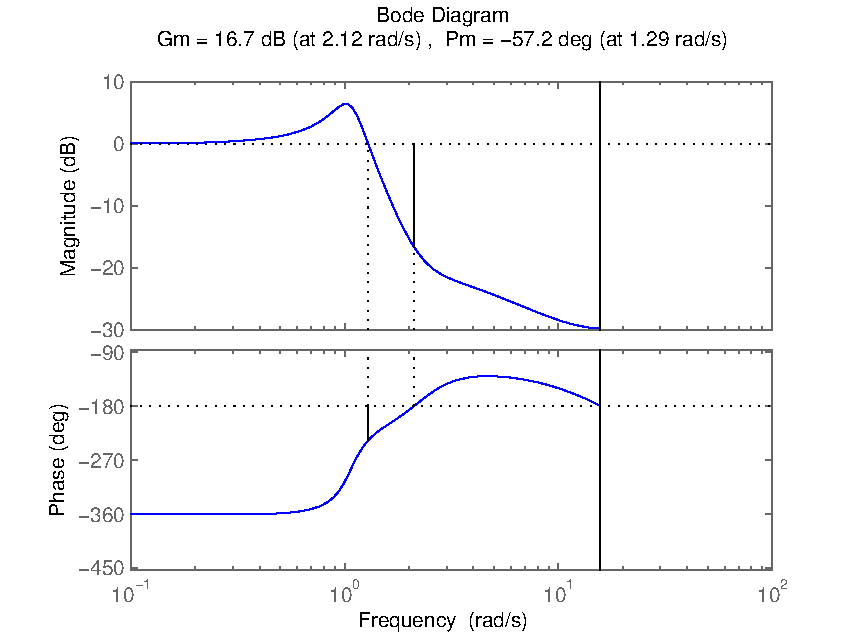
\includegraphics[width=\textwidth]{figures/runningexample_bd0.pdf}
        \caption{Original controller~\cite{DBLP:conf/hybrid/WangGRJF16}}
        \label{fig:original}
    \end{subfigure}
    ~
    \begin{subfigure}[b]{0.4\textwidth}
        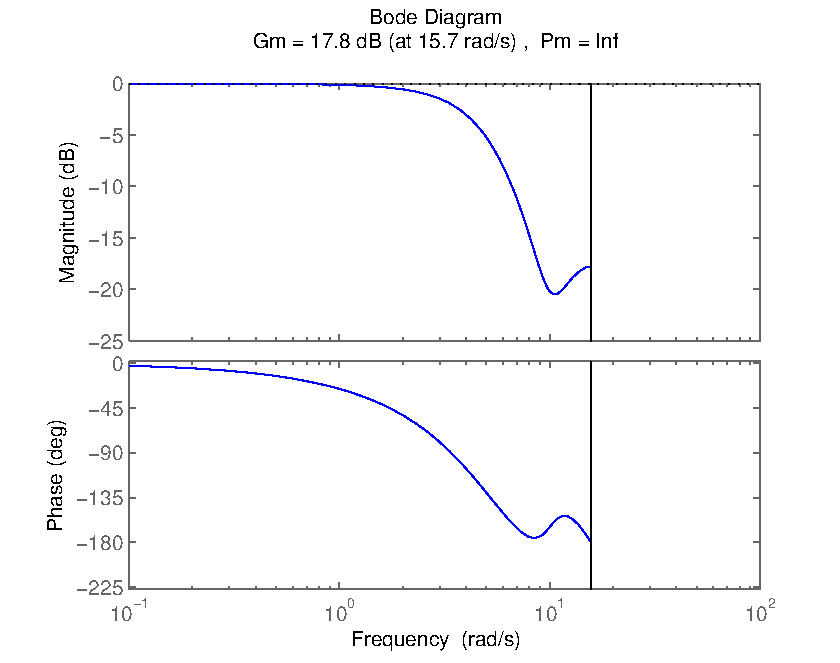
\includegraphics[width=\textwidth]{figures/runningexample_bd2.pdf}
        \caption{Controller synthesized by \tool}
        \label{fig:cegiscontroller}
    \end{subfigure}
    \caption{Bode diagram for original controller in~\cite{DBLP:conf/hybrid/WangGRJF16} 
    and for newly synthesized closed-loop system}\label{fig:bode}
\end{figure}

Figure~\ref{fig:step} illustrates the step responses of the closed-loop
system with the original controller represented by
Eq.~\eqref{Eq:running-example-controller} (Figure~\ref{fig:step0}), the
first (Figure~\ref{fig:step1}) and final (Figure~\ref{fig:step2}) candidate
solutions provided by \tool.  The step response in Figure~\ref{fig:step0}
confirms the stability loss if we consider FWL effects.  
Figure~\ref{fig:step1} shows that the first candidate controller is able to
stabilize the closed-loop system without uncertainties, but it is rejected
during the {\sc precision} phase by \tool since this solution is not
considered to be sound.  Finally, Figure~\ref{fig:step2} shows a stable
behavior for the final (sound) solution, which presents a lower settling
time (hence the noticeable digitazion effects).

\begin{figure*}
    \centering
    \begin{subfigure}[b]{0.3\textwidth}
        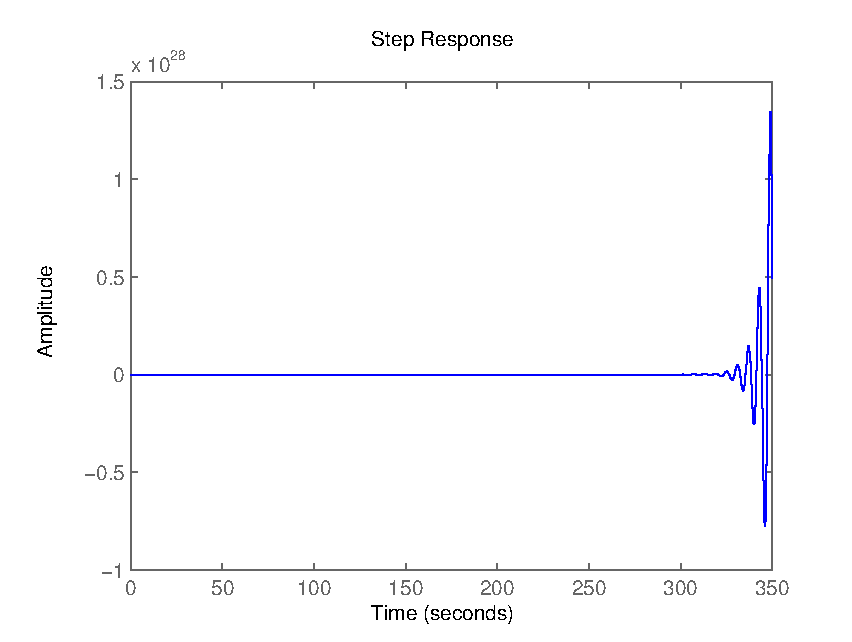
\includegraphics[width=\textwidth]{figures/runningexample_step0.pdf}
        \caption{Original controller}
        \label{fig:step0}
    \end{subfigure}
    ~
    \begin{subfigure}[b]{0.3\textwidth}
        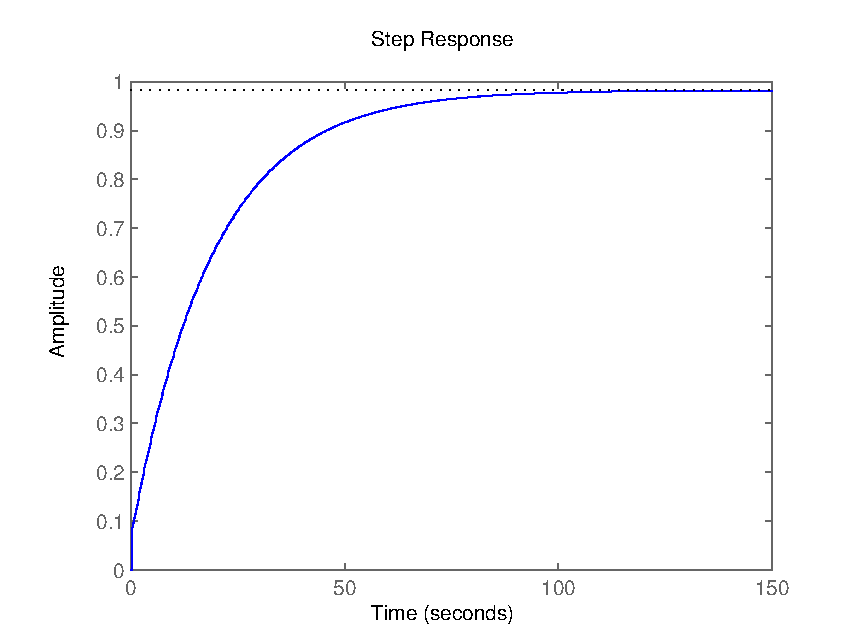
\includegraphics[width=\textwidth]{figures/runningexample_step1.pdf}
        \caption{First solution by \tool}
        \label{fig:step1}
    \end{subfigure}
    ~
    \begin{subfigure}[b]{0.3\textwidth}
        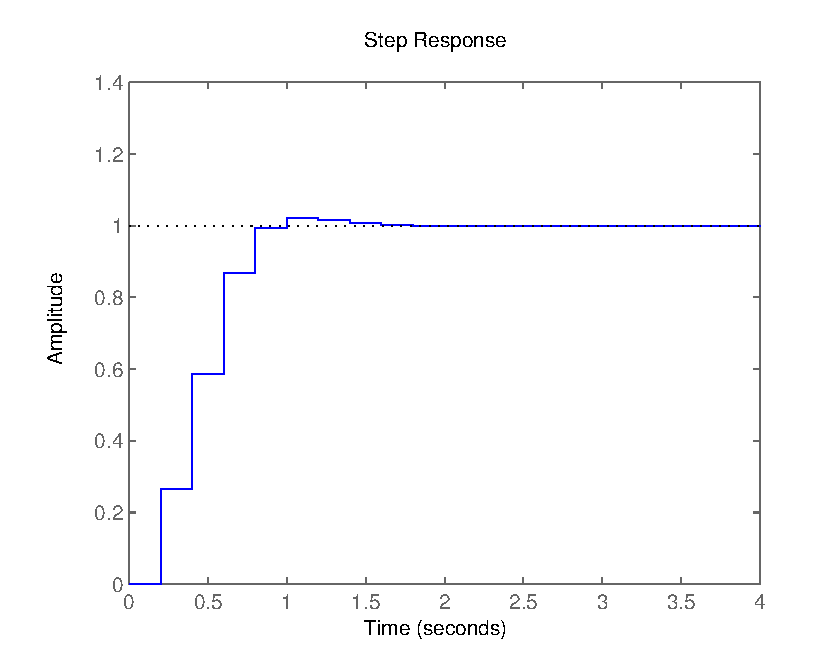
\includegraphics[width=\textwidth]{figures/runningexample_step2.pdf}
        \caption{Final solution by \tool}
        \label{fig:step2}
    \end{subfigure}
    \caption{Step responses for original~\cite{DBLP:conf/hybrid/WangGRJF16}
             closed-loop system with FWL effects and for each
             {\sc synthesize} iteration of \tool}\label{fig:step}
\end{figure*}

%%%%%%%%%%%%%%%%%%%%%%%%%%%%%%%%%%%%%%%%%%%%%%%%%%%%%%%%%%%%%%%%%%%%%%%%%%%%%%%%%%%%%%
\section{Experimental Evaluation}\label{sec:experiments}

%This section is split into three parts. Section~\ref{experimental-setup}
%discusses the experimental setup and our benchmarks, while
%Section~\ref{experimental-objectives} describes the experimental objectives. 
%Section~\ref{experimental-results} presents the experimental results
%obtained on the benchmarks with our tool \tool.

%---------------------------------
\subsection{Description of the Benchmarks}
\label{experimental-setup}
%---------------------------------

The first set of benchmarks uses the discrete model $G_1(z)$ of a cruise control
system for a car, and accounts for rolling friction, aerodynamic drag, and
the gravitational disturbance force~\cite{Astrom08}. 
%The plant model is given as follows:
%
%\begin{equation}
%\label{cruise-control-c1}
%G_1(z)=\frac{0.0264}{z-0.998} \nonumber
%\end{equation} 
%
The second set of benchmarks considers the discrete model $G_2(z)$ 
of a simple spring-mass damper plant~\cite{DBLP:conf/hybrid/WangGRJF16}. 
%where the discrete 
%plant dynamics is represented by the following $z$-expression:
%
%\begin{equation}
%\label{spring-mass-damper-g}
%G_2(z)=\frac{5\times{10^{-5}}z + 5\times{10^{-5}}}{z^2 - 2z + 1.0001}. \nonumber
%\end{equation} 
%
A third set of benchmarks uses the discrete model $G_{3}(z)$ for satellite attitude 
dynamics~\cite{Franklin15}, which require attitude control
for orientation of antennas and sensors w.r.t.~Earth.
The fourth set of benchmarks presents an alternative discrete model $G_4(z)$ 
of a cruise control system~\cite{DBLP:conf/hybrid/WangGRJF16}. 
%The satellite
%attitude control is typically used for three-axis attitude tracking, but
%here we consider only one axis at a time.  
%The motion equation for the
%one-axis system, disregarding disturbance torques, is given by
%
%\begin{equation}
%\label{eq:satelliteode}
%I\cdot \ddot{\theta} = \tau_{C}, 
%\end{equation}
%
%\noindent where $I$ is the satellite inertia moment about its mass
%center, $\tau_{C}$ is the control torque applied by the thrusters, and
%$\theta$ is the controlled attitude angle.  Normalizing
%Eq.~\eqref{eq:satelliteode} by defining the control signal
%$u=\frac{\tau_{C}}{I}$ and taking the Laplace transform, the following
%$s$-domain transfer function $G(s)$ is obtained:
%
%\begin{equation}
%\label{eq:satellitetf}
%G_{3}(s)=\frac{\theta(s)}{u(s)}=\frac{1}{s^2},
%\end{equation}
%
%\noindent Using the ZOH discretization defined in Eq.~\eqref{eq:pulsetf}, 
%we get the following $z$-domain model:
%
%\begin{equation}
%G_{3}(z)= \frac{T^{2}}{2} \frac{z+1}{(z+1)^{2}}. \nonumber
%\end{equation}
%
%
%\begin{equation}
%\label{exampleA}
%G_{4}(s)=\frac{s-1}{s^{2}-s-2},
%\end{equation}
%
%\noindent We can obtain $G_{4}(z)$ using the ZOH discretization defined
%in Eq.~\eqref{eq:pulsetf} with three different sample times ($0.1$, $0.05$,
%and $0.03$ seconds), respectively, as follows:
%
%\begin{equation}
%\label{exampleA-sampletime1}
%G_{4a}(z)=\frac{0.100342181002722z - 0.110876810062963}{1.0z^{2} - 2.12624017619613z + 1.10517091807565}, \nonumber
%\end{equation}
%
%
%\begin{equation}
%\label{exampleA-sampletime2}
%G_{4b}(z)=\frac{0.0500422033454653z - 0.0526068264456340}{1.0^{2} - 2.05640034257636z + 1.05127109637602}, \nonumber
%\end{equation}
%
%\begin{equation}
%\label{exampleA-sampletime3}
%G_{4c}(z)=\frac{0.0300090687252212z - 0.0309228417953966}{1.0^{2} - 2.03228208009387z + 1.03045453395352}. \nonumber
%\end{equation}
%
The fifth and sixth set of benchmarks describe the discrete model 
of a DC servo motor velocity dynamics~\cite{exampleCAD,Tan01}. 
%
The seventh set of benchmarks contains a well-studied discrete  
non-minimal phase model $G_{7}(z)$. As known, non-minimal phase model offers 
additional difficulties for the design of stable controllers~\cite{Doyle:1991:FCT:574259}. 
%
%The fifth set of benchmarks contains the \textit{DC Motor Rate} discrete model $G_{5}(z)$, which 
%describes the angular velocity of a DC Motor plant~\cite{Franklin15}. 
%
%\begin{equation}
%\label{DC-Motor-Rate}
%G_{5}(z)=\frac{ 0.1898z + 1.8027\times{10^{-4}}}{1.0z^{2} -0.9012z -1.0006\times{10^{-16}}}. \nonumber
%\end{equation}
%
The eighth set of benchmarks describes the discrete model $G_{8}(z)$ for the \textit{Helicopter Longitudinal Motion},
which provides the longitudinal motion dynamics of a helicopter~\cite{Franklin15}. 
%
%\begin{equation}
%\label{Helicopter-Longitudinal-Motion}
%G_{6}(z)=\frac{15.1315z^{2} + 17.8600z + 17.4549}{z^{3} -2.6207z^{2} + 2.3586z -0.6570}. \nonumber
%\end{equation}
%
The ninth  set of benchmarks contains the discrete model $G_{9}(z)$ for the known \textit{Inverted Pendulum}, which 
describes a pendulum dynamics with its center of mass above its pivot point~\cite{Franklin15}. 
%
%\begin{equation}
%\label{Inverted-Pendulum}
%G_{7}(z)=\frac{0.0263z^{2} + 0.0143z -0.0383}{z^{4} -4.2553z^{3} + 6.5105z^{2} -4.2553z + 1}. \nonumber
%\end{equation}
%
The tenth set of benchmarks contains the \textit{Magnetic Suspension} discrete model $G_{10}(z)$, which describes the dynamics of a mass that levitates with support only of a magnetic field~\cite{Franklin15}. 
%
%\begin{equation}
%\label{Magnetic-Suspension}
%G_{8}(z)=\frac{6.769\times{10^{13}}z + 6.784\times{10^{13}}}{z^{2} -5.415\times{10^{13}}z + 4.23\times{10^{11}}}. \nonumber
%\end{equation}
%The ninth set of benchmarks contains the \textit{1/4 Car Suspension} discrete model $G_{9}(z)$,
%which represents the dynamics of a single wheel suspension plant, {\it i.e.}, a system that connects a car to a wheel and allows relative motion between both %parts~\cite{Franklin15}.
%
%\begin{equation}
%\label{Car-Suspension}
%G_{8}(z)=\frac{0.25z^{3} + 0.5z^{3} + 0.25z -5.7065\times{10^{-10}}}{z^{3} + 6.8455\times{10^{-9}}z^{2} + 3.3925\times{10^{-17}}z - 3.4667\times%{10^{-94}}}. \nonumber
%\end{equation}
%
The eleventh set of benchmarks contains the \textit{Computer Tape Driver} discrete model $G_{11}(z)$, which 
describes a system to read and write data on a storage device~\cite{Franklin15}.
%
%\begin{equation}
%\label{Computer-Tape-Driver}
%G_{10}(z)=\frac{0.0200z -3.8303\times{10^{-176}}}{1.0z -4.6764\times{10^{-166}}}. \nonumber
%\end{equation}
%
The last set of benchmarks considers a discrete model $G_{12}(z)$ 
that is typically used for evaluating stability
margins and controller fragility~\cite{bhattacharyya97, keel_Bhattacharyya_examples}.

Additional benchmarks were created for the \textit{Cruise Control System}, \textit{Springer-mass damper}, and \textit{Satellite} considering parametric additive in the nominal plant model  (represented by $\Delta_{p}\vec{G}$ in Eq.~\eqref{digital_plant_tf}). The uncertainties are deviations bounded to a maximum magnitude of $0.5$ in each coefficient. These uncertain models are respectively represented by $G_{1b}(z)$, $G_{2b}(z)$, $G_{3b}(z)$, and $G_{3d}(z)$. 

All experiments have been conducted on a 12-core 2.40\,GHz Intel Xeon E5-2440
with 96\,GB of RAM and Linux OS.  All times given are wall clock times in
seconds, as measured by the UNIX date command.  For the two-stage verification 
engine in Figure~\ref{fig:CEGIS} we have applied a timeout of $8$ hours per benchmark, 
whereas $24$ hours have been set for the approach using a one-stage engine. 

%---------------------------------
\subsection{Objectives}
\label{experimental-objectives}
%---------------------------------

Using the closed-loop control system benchmarks given in
Section~\ref{experimental-setup}, our experimental evaluation aims to answer
two research questions:
%
\begin{enumerate}

\item[RQ1] \textbf{(performance)} does the CEGIS approach generate a 
FWL digital controller in a reasonable amount of time?

\item[RQ2] \textbf{(sanity check)} are the synthesized controllers sound
and can their stability be confirmed outside of our model?

\end{enumerate}

%---------------------------------
\subsection{Results}
\label{experimental-results}
%---------------------------------

We give the run-times required to synthesize a stable controller for each
benchmark in Table~\ref{tab:results}.  Here, \textit{Plant} is the discrete
or continuous plant model, \textit{Benchmark} is the name of the employed
benchmark, \textit{I} and \textit{F} represent the number of integer and
fractional bits of the stable controller, respectively, 
while the two right columns display the total time (in seconds) required to synthesize a stable controller
for the given plant. 

For the majority of the benchmarks, the conjecture explained in
Section~\ref{synthesis-elements} holds and the two-stage verification 
engine is able to find a stable solution in less than one minute for half
of the benchmarks. This is possible if the inductive solutions need to be 
refined with few counterexamples and increments of the fixed-point precision.  
However, the benchmark \emph{SatelliteB2} with uncertainty ($G_{3b}$) has 
required too many counterexamples to refine its solution.  
For this particular case, the one-stage engine is able to complement the
two-stage approach and synthesize a solution instead.  It is important to
reiterate that the one-stage verification engine does not take advantage of
the inductive conjecture inherent to CEGIS, but instead fully explores the
counterexample space in one SAT instance.  As expected, this approach is 
significantly slower on average and is only useful for benchmarks where 
the CEGIS approach requires too many counterexample refinement iterations
such that exploring all counterexamples in a single SAT instance performs better.
Our results suggest an average performance difference of at least two orders
of magnitude between the two engines, leading to the one-stage engine timing
out on the majority of our benchmarks.  Table~\ref{tab:results}
lists the results for both engines, where in $16$ out of $23$
benchmarks, the two-stage engine is faster.

\begin{table}
\centering
\scalebox{0.8}{
\begin{tabular}{| r | c | l | r r || r | r |}
\hline
\# & Plant  & Benchmark                  & $I$ & $F$
   & 2-stage & 1-stage
    \\\hline\hline
1  & $G_{1a}$  & CruiseControl02
            &   4 &  16 & \textbf{12\,s}   & 67\,s     \\
2  & $G_{1b}$  & CruiseControl02$^\dagger$
            &   4 &  16 & 14600\,s   & \textbf{52\,s}     \\
3  & $G_{2a}$  & SpgMsDamper
            &  15 &  16 & \textbf{52\,s}   & 318\,s     \\
4  & $G_{2b}$  & SpgMsDamper$^\dagger$
            &  15 &  16 & \xmark  & \xmark    \\
5  & $G_{3a}$  & SatelliteB2
            &   3 &   7 & \textbf{36\,s}    & \xmark     \\
6  & $G_{3b}$  & SatelliteB2$^\dagger$
            &   3 &   7 & \xmark  & \textbf{4111\,s}  \\
7  & $G_{3c}$  & SatelliteC2
            &   3 &   5 & \textbf{3\,s}    & 205\,s    \\
8  & $G_{3d}$  & SatelliteC2$^\dagger$
            &   3 &   5 & \textbf{50\,s}  & 1315\,s    \\
9  & $G_4$  & Cruise
            &   3 &   7 & 1\,s  & 1\,s    \\
10 & $G_5$  & DCMotor
            &   3 &   7 & \textbf{1\,s}  & 10\,s    \\
11 & $G_6$  & DCServomotor
            &   4 &  11 & \textbf{46\,s}  & \xmark    \\
12 & $G_7$  & Doyleetal
            &   4 &  11 & \textbf{8769\,s}  & \xmark    \\
13 & $G_8$  & Helicopter
            &   3 &   7 & \textbf{44\,s}  & \xmark    \\
14 & $G_9$  & Pendulum
            &   3 &   7 & \textbf{1\,s}  & 14826\,s    \\
15 &$G_{10}$& Suspension
            &   3 &   7 & \textbf{1\,s}  & 5\,s    \\
16 &$G_{11}$& Tapedriver
            &   3 &   7 & 1\,s  & 1\,s    \\
17 &$G_{12a}$& a\_ST1\_IMPL1
            &  16 &   4 & \textbf{11748\,s} & \xmark   \\
18 &$G_{12a}$& a\_ST1\_IMPL2
            &  16 &   8 & \textbf{351\,s}  & \xmark   \\
19 &$G_{12a}$& a\_ST1\_IMPL3
            &  16 &  12 & \textbf{8772\,s}   & \xmark   \\
20 &$G_{12b}$& a\_ST2\_IMPL1
            &  16 &   4 & \textbf{1128\,s}  & \xmark   \\
21 &$G_{12b}$& a\_ST2\_IMPL2
            &  16 &   8 & \xmark  & \xmark    \\
22 &$G_{12b}$& a\_ST2\_IMPL3
            &  16 &  12 & \textbf{15183\,s} & \xmark   \\ 
23 &$G_{12c}$& a\_ST3\_IMPL1
            &  16 &   4 & \xmark & \xmark   \\\hline
\end{tabular}}\\[0.2ex]
\caption{\tool results ({\xmark} = time-out, $\dagger$ = 
uncertainty)
\label{tab:results}}
\end{table}
%---------------------------------

The presence of uncertainty in some particular benchmarks ($2$, $4$, $6$, and $8$)  
leads to harder verification conditions to be checked 
by the {\sc verify} phase, which thus influences the overall synthesis time.   
However, considering the faster engine for each benchmark (marked as bold in Table~\ref{tab:results}), 
the median run-time amounts to $48$\,s, implying that \tool can synthesize 
half of the controllers in less than one minute. Overall, the average fastest synthesis 
time considering both engines is approximately $42$ minutes.  We
consider these times short enough to be of practical use to control
engineers, and thus affirm RQ1.  We further observe that the approach using
the two-stage verification engine is able to synthesize stable controllers
in $19$ out of the $23$ benchmarks, and can be complemented using the
one-stage engine, which is faster for two benchmarks where the inductive
conjectures fail.  Both verification engines together enable controller
synthesis for $20$ out of $23$ benchmarks.  For the remaining benchmarks
our approach failed to synthesize a stable controller within the time
limits.  This can be addressed by either increasing either the time limit
or the fixed-point word widths considered, or by using floating-point
arithmetic instead.  The synthesized controllers have been confirmed to be stable
outside of our model representation using MATLAB, positively answering RQ2. 
A~link to the full experimental environment, including scripts to reproduce
the results, all benchmarks and the \tool tool, is provided in the
footnote.\footnote{\url{http://www.cprover.org/DSSynth/experiment.tar.gz}\\ 
CBMC (SHA-1 hash) version: \\ 
7a6cec1dd0eb8843559591105235f1f2c4678801}

%--------------------------------------
\subsection{Threats to Validity and Generalizations}
%--------------------------------------

We have reported a favourable assessment of \tool over a diverse set of real-world
benchmarks. Nevertheless, this set of benchmarks is limited within the
scope of this paper and \tool's performance 
%may not generalize to other benchmark scenarios. This can 
needs to be addressed by expanding the benchmarks set
in future experiments.

Furthermore, our approach to select suitable FWL word widths to model
plant behavior employs a heuristic based on user-provided controller
word-width specifications.  Given the encouraging results of our benchmarks,
this heuristic appears to be strong enough for the current benchmark set,
but this may not generalize.  Further experiments towards determining
suitable plant FWL configurations may thus be necessary in future work.

Finally, the experimental results obtained using \tool for stability
properties may not generalize to other properties.  The inductive nature of
the two-stage back-end of \tool increases performance significantly compared
to the one-stage back-end, but this performance benefit introduced by CEGIS 
inductive generalizations may not be observed for other controller 
properties.  Additional experiments are necessary to confirm that the
performance of our inductive synthesis approach can be leveraged in those
scenarios.

%%%%%%%%%%%%%%%%%%%%%%%%%%%%%%%%%%%%%%%%%%%%%%%%%%%%%%%%%%%%%%%%%%%%%%%%%%%%%%%%%%%%%%
\section{Related Work}\label{sec:related}

\paragraph{Robust Synthesis of Linear Systems} 

The problem of parametric control synthesis based on stability measures for
continuous Linear Time Invariant (LTI) Single Input-Single Output (SISO)
systems has been researched for several decades.  On a theoretical level it
is a solved problem~\cite{wonham1967pole}, for which researchers
continuously seek better results for a number of aspects in addition to
stability.  A vast range of pole placement techniques such as Moore's
algorithm for eigenstructure assignment~\cite{klein1977eigenvalue} or the
more recent Linear Quadratic Regulator (LQR)~\cite{bemporad2002explicit}
have been used in several studies with increasing degrees of success to
ensure stability.  The latter approach highlights the importance of
conserving energy during the control process, which results in lower running
costs.  Since real systems are subject to tolerance and noise as well as the
need for economy, more recent studies focus on the problem of achieving
robust stability with minimum gain~\cite{schmid2014unified,
konigorski2012pole}.  However, when applied with the aim of synthesising a
digital controller, many of these techniques lack the ability to produce
sound or stable results because they disregard the effects of quantization
and rounding.  Recent papers on implementations/synthesis of LTI digital
controllers~\cite{das2013lqr, ghosh2013fpga} focus on time discretization,
failing to account for these error-inducing effects and can result in digital 
systems that are unstable even though they have been proven to be
robustly stable in a continuous space.  

\paragraph{Formal Verification of Linear Digital Controllers} 

Researchers in formal verification of control systems have studied various
effects of discretizing the dynamics, including delayed
response~\cite{Duggirala2015}, and Finite Word Length (FWL) semantics \cite{Anta:2010:AVC:1879021.1879024} 
with the goal to either verify~\cite{daes20161} or to optimize~\cite{oudjida2014design} 
given implementations.

There are two different problems that arise from FWL semantics.  The first
is the error in the dynamics caused by the inability to represent the exact
state of the physical system while the second relates to rounding errors
during computation.  In~\cite{fialho1994stability}, a stability measure
based on the error of the digital dynamics ensures that the deviation
introduced by FWL does not make the digital system unstable.  A~recent
approach~\cite{DBLP:journals/automatica/WuLCC09} uses the $\mu$-calculus to
directly model the digital controller so that the selected parameters are
stable by design.  Most work in verification focuses on finding a correct
variant of a known controller, looking for optimal parameter
representations using FWL, but ignore the effects of rounding errors due to
issues of mathematical tractability.  The analyses
in~\cite{DBLP:conf/hybrid/RouxJG15,DBLP:conf/hybrid/WangGRJF16} rely on an
invariant computation on the discrete system dynamics using Semi-Definite
Programming (SDP).  While the former uses BIBO properties to determine
stability, the latter uses Lyapunov-based quadratic invariants.  In both
cases, the SDP solver uses floating-point arithmetic and soundness is
checked by bounding the error.  An alternative approach is taken
by~\cite{park2016scalable}, where the verification of existing code is
performed against a known model by extracting an LTI model of the code
through symbolic execution.  In order to account for rounding errors, an
upper bound is introduced in the verification phase.  If~the error of the
implementation is lower than this tolerance level, then the verification is
successful.

\paragraph{Robust Synthesis of FWL Digital Controllers}

There is no technique in the existing literature for automatic synthesis of
fixed-point digital controllers that considers FWL effects.
%  Parameter
%synthesis tools such as~\cite{cimatti2013parameter} use bounded model
%checking and fixed-point computations to compute parameters based on
%user-defined specifications, but they often operate in the continuous domain
%and have no direct means of evaluating robustness.

Other tools such as~\cite{economakos2016automated} are aimed at
robust stability problems, but they fail to take the FWL effects into
account.  In order to provide a correct-by-design digital controller,
\cite{alur2016compositional} requires a user-defined finite-state
abstraction to synthesize a digital controller based on high-level
specifications.  While this approach overcomes the challenges presented by
the FWL problem, it still requires error-prone user intervention. 
A~different solution that uses FWL as the starting point is an approach that
synthesizes word lengths for known control problems~\cite{jha2013swati};
however, this provides neither an optimal result nor a comprehensive
solution for the problem.

\paragraph{The CEGIS Architecture}

Program synthesis is the problem of computing correct-by-design programs
from high-level specifications, and algorithms for this problem have made
substantial progress in recent years.  One such
approach~\cite{itzhaky2010simple} inductively synthesizes invariants to
generate the desired programs.

Program synthesisers are an ideal fit for synthesis of parametric
controllers since the semantics of programs capture effects such as FWL
precisely.  In~\cite{DBLP:conf/cdc/RavanbakhshS15}, the authors use CEGIS
for the synthesis of switching controllers for stabilizing continuous-time
plants with polynomial dynamics.  The work extends to its application on
affine systems, finding its major challenge in the hardness of solving
linear arithmetic with the state-of-the-art SMT solvers.  Since this
approach uses switching states instead of linear dynamics in the digital
controller, it entirely circumvents the FWL problem.  It is also not
suitable for the kind of control we seek to synthesize.  We require a
combination of a synthesis engine with a control verification tool that
addresses the challenges presented here in the form of FWL effects and
stability measures for LTI SISO controllers.  We take the former
from~\cite{DBLP:conf/lpar/DavidKL15} and the latter from~\cite{daes20161}
while enhancing the procedure by evaluating the quantization effects of the
Hardware interfaces (ADC/DAC) to obtain an accurate discrete-time FWL
representation of the continuous dynamics.
 
%In \cite{DBLP:journals/corr/PakmehrWJVF13}, Pakmehr et al.  design a control software verification framework for gas turbine engines.

%%%%%%%%%%%%%%%%%%%%%%%%%%%%%%%%%%%%%%%%%%%%%%%%%%%%%%%%%%%%%%%%%%%%%%%%%%%%%%%%%%%%%%
\section{Conclusions}\label{sec:conclusions}

We have presented a CEGIS-based approach implemented in a tool called \tool,
which uses inductive synthesis in conjunction with an algorithm for
verifying robust closed-loop stability that addresses plant variations as
interval sets as well as FWL uncertainties in digital controllers.  The
novelty in our approach is that it is fully automated and algorithmically
and numerically sound.  In particular, \tool marks the first use of the
CEGIS that handles plants with uncertain models and FWL effects over the
digital controller.  Implementing this architecture efficiently requires
adjusting the traditional CEGIS refinement loop to the use of a two-stage
verification engine: here, the first stage performs fast, but potentially
unsound fixed-point operations, whereas the second stage restores soundness
by validating the operations performed by the first stage using interval
arithmetic.  Our experimental results show that \tool is able to synthesize
stable controllers in most benchmarks within a reasonable amount of time
fully automatically.  Future work will be the extension of this CEGIS-based
approach to further classes of systems, including those with state space. 
We will also consider performance requirements while synthesizing the
digital controller.

\bibliographystyle{abbrv}
\bibliography{paper}  

%APPENDICES are optional
%\balancecolumns
%\appendix
%Appendix A

\end{document}
